\documentclass[11pt, a4paper]{article}

% --- Typography & Geometry ---
\usepackage[a4paper, left=1.25in, right=1.25in, top=1.4in, bottom=1.25in, headheight=15pt, headsep=20pt]{geometry}
\usepackage[T1]{fontenc}
\usepackage{newtxtext}
\usepackage{newtxmath}
\usepackage{microtype}

\usepackage[
    backend=biber,
    style=phys,          
    articletitle=false,  
    biblabel=brackets   
]{biblatex}
% --- Math & Physics Packages ---
\usepackage{amsmath}
\usepackage{braket}

% --- Graphics & Floats ---
\usepackage{graphicx}
\usepackage[section]{placeins}
\usepackage[labelfont=bf, font=small, margin=12pt]{caption}

% --- Code & Appendices ---
\usepackage{appendix}
\usepackage{listings}
\usepackage{xcolor}

% --- Code Listing Setup ---
\definecolor{codegreen}{rgb}{0.13,0.55,0.13}
\definecolor{codegray}{rgb}{0.5,0.5,0.5}
\definecolor{codepurple}{rgb}{0.58,0,0.82}
\definecolor{backcolour}{rgb}{0.96,0.96,0.96}

\lstset{
    language=Python,
    backgroundcolor=\color{backcolour},
    commentstyle=\color{codegreen}\itshape,
    keywordstyle=\color{blue}\bfseries,
    numberstyle=\tiny\color{codegray},
    stringstyle=\color{codepurple},
    basicstyle=\ttfamily\small,
    breakatwhitespace=false,
    breaklines=true,
    captionpos=b,
    keepspaces=true,
    numbers=left,
    numbersep=10pt,
    showspaces=false,
    showstringspaces=false,
    showtabs=false,
    tabsize=4,
    frame=none, % Removed the harsh top/bottom rules
    xleftmargin=15pt,
    xrightmargin=5pt,
    aboveskip=1.5em,
    belowskip=1.5em
}

% --- Microtypography & Page Breaks ---
\clubpenalty=10000
\widowpenalty=10000
\displaywidowpenalty=10000


% --- Hyperlinks ---
\usepackage[colorlinks=true,
            linkcolor=blue!60!black,
            citecolor=blue!60!black,
            urlcolor=blue!60!black]{hyperref}

\usepackage[capitalize,nameinlink]{cleveref}
\usepackage{subcaption}
\usepackage[export]{adjustbox}

\renewcommand{\topfraction}{.85}
\renewcommand{\bottomfraction}{.7}
\renewcommand{\textfraction}{.15}
\renewcommand{\floatpagefraction}{.66}

% --- Headers and Footers ---
\usepackage{fancyhdr}
\pagestyle{fancy}
\fancyhf{} % Clear all default headers and footers
\fancyhead[L]{\small\sffamily\leftmark} % Section name on the left
\fancyhead[R]{\small\sffamily The Su--Schrieffer--Heeger (SSH) Model} % Short title on the right
\fancyfoot[C]{\thepage} % Page number at the bottom center
\renewcommand{\headrulewidth}{0.4pt} % Subtle line under header
\setlength{\headheight}{14pt}
\usepackage{booktabs}\addbibresource{references.bib}
\begin{document}
\pagestyle{fancy}


\begin{titlepage}
    \centering        
    {\Huge \textbf{A Theoretical and Numerical Study of the Su–Schrieffer–Heeger Model}}\\[1.5cm]
    
    {\Large \textbf{Summer Research Internship Report}}\\[3cm]
    
    \vfill
    % Two-column layout for Student and Supervisor
    \begin{minipage}{0.45\textwidth}
        \begin{flushleft} \large
            \emph{Prepared by:}\\[0.2cm]
            \textbf{Vijay Vedanth Vemula}\\
            BS--MS Student\\
            IISER Tirupati
        \end{flushleft}
    \end{minipage}
    \hfill
    \begin{minipage}{0.45\textwidth}
        \begin{flushright} \large
            \emph{Supervised by:}\\[0.2cm]
            \textbf{Dr.~Panch Ram}\\
            Department of Physics\\
            IIT (BHU), Varanasi
        \end{flushright}
    \end{minipage}
    
    \vfill
    
    {\large \textbf{Summer 2026}}\\[1cm]
\end{titlepage}

\clearpage
\hypersetup{pageanchor=false}

\pagenumbering{roman}
\setcounter{page}{1}

\tableofcontents

\clearpage
\hypersetup{pageanchor=true}

\pagenumbering{arabic}
\setcounter{page}{1}
\pagestyle{fancy}

\section{Introduction}
The Su--Schrieffer--Heeger (SSH) model is a one-dimensional tight-binding model that serves as one of the simplest theoretical frameworks for studying topological phases of matter.
Originally introduced to describe the electronic properties of polyacetylene \cite{ssh1979}, the model has since become one of the canonical examples for understanding topological band theory and one-dimensional topological insulators \cite{asboth2015}.
Despite its simple structure, the SSH model exhibits non-trivial topological behaviour and provides an accessible platform for understanding concepts such as energy bands, topological phase transitions, and edge states, which are central topics in the study of topological insulators \cite{hasan2010,qi2011}.
These notes present the derivation of the SSH model starting from its real-space tight-binding Hamiltonian.
The Hamiltonian is expressed in matrix form for a finite lattice and subsequently reformulated using the tensor-product representation of the unit-cell and sublattice degrees of freedom.
By imposing periodic boundary conditions and applying Bloch's theorem, the bulk momentum-space Hamiltonian is obtained, from which the energy dispersion relation is derived.
Finally, the Hamiltonian is expressed in terms of Pauli matrices, leading to the vector representation that forms the basis for describing the topological properties of the model.~\cite{asboth2015}

\section{The Su--Schrieffer--Heeger Model}
\label{sec:ssh_model}
\begin{figure}[htbp]
    \centering
    
\includegraphics[width=\linewidth]{Figures/ssh_chain_bulkedge.pdf}
    \caption{Geometry of the Su--Schrieffer--Heeger (SSH) model.
Each unit cell consists of two sublattice sites, A (grey) and B (white), with alternating intracell ($v$) and intercell ($w$) hopping amplitudes.
Reproduced from Asbóth \textit{et al}~\cite{asboth2015}.}
    \label{fig:ssh_chain}
\end{figure}

\subsection{Real-Space Tight-Binding Hamiltonian}
The Su--Schrieffer--Heeger (SSH) model describes a one-dimensional lattice composed of $N$ unit cells, with each unit cell containing two inequivalent lattice sites belonging to sublattices $A$ and $B$, as shown in \cref{fig:ssh_chain}.
The model assumes that a particle can hop only between nearest-neighbour sites.
Due to the alternating bond strengths, two distinct hopping amplitudes are introduced: the intracell hopping amplitude $v$, which couples the A and B sites within the same unit cell, and the intercell hopping amplitude $w$, which couples the B site of one unit cell to the A site of the neighbouring unit cell.~\cite{ssh1979,asboth2015}
Within the tight-binding approximation \cite{ashcroft1976,asboth2015}, the basis states are denoted by $|m,A\rangle$ and $|m,B\rangle$, representing a particle localized on the A or B site of the $m^{\text{th}}$ unit cell, respectively.
Neglecting the on-site potentials and restricting the hopping to nearest neighbours, the real-space Hamiltonian of the SSH model is written as
\begin{equation}
\label{eq:ssh_hamiltonian}
    \hat{H}= v\sum_{m=1}^{N} \left( |m,B\rangle \langle m,A| + \mathrm{h.c.} \right) + w \sum_{m=1}^{N-1}\left( |m+1,A\rangle \langle m,B| + \mathrm{h.c.} \right)
\end{equation}
where $\mathrm{h.c.}$ represents the Hermitian conjugate.

\subsection{Matrix Representation of the Hamiltonian}
To obtain an explicit matrix representation of the SSH Hamiltonian, we consider a finite chain and express the Hamiltonian in a localized basis.
For a chain consisting of $N$ unit cells, the Hilbert space has dimension of $2N$, since each unit cell contains two sublattice sites.
As an example, we first consider a chain with $N=4$ unit cells.
The basis states are chosen as $\{|1,A\rangle,|1,B\rangle,|2,A\rangle,|2,B\rangle,|3,A\rangle,|3,B\rangle,|4,A\rangle,|4,B\rangle\}$
Using \cref{eq:ssh_hamiltonian}, the action of the Hamiltonian on each basis state is obtained as 
\begin{align*}
    \hat H |1,A\rangle &= v|1,B\rangle,\\
    \hat H|1,B\rangle &= v|1,A\rangle + w|2,A\rangle,\\
    \hat H|2,A\rangle &= v|2,B\rangle + w|1,B\rangle,\\
    \hat H|2,B\rangle &= v|2,A\rangle + w|3,A\rangle,\\
    \hat H|3,A\rangle &= v|3,B\rangle + w|2,B\rangle,\\
    \hat H|3,B\rangle &= v|3,A\rangle + w|4,A\rangle,\\
    \hat H|4,A\rangle &= v|4,B\rangle + w|3,B\rangle,\\
    \hat H|4,B\rangle &= v|4,A\rangle
\end{align*}
Each equation gives one column of the Hamiltonian matrix in the chosen basis. For example,
$\hat{H}|1,A\rangle = v|1,B\rangle$ means that the first column has only one nonzero element, $H_{21}=v$, while $\hat{H}|1,B\rangle = v|1,A\rangle + w|2,A\rangle$ gives the second column $H_{12}=v$ and $H_{32}=w$.
Repeating this procedure for all basis states gives
\begingroup
\renewcommand{\arraystretch}{1.15}
\begin{equation*}
H=
\begin{pmatrix}
0 & v & 0 & 0 & 0 & 0 & 0 & 0\\
v & 0 & w & 0 & 0 & 0 & 0 & 0\\
0 & w & 0 & v & 0 & 0 & 0 & 0\\
0 & 0 & v & 0 & w & 0 & 0 & 0\\
0 & 0 & 0 & w & 0 & v & 0 & 0\\
0 & 0 & 0 & 0 & v & 0 & w & 0\\
0 & 0 & 0 & 0 & 0 & w & 0 & v\\
0 & 0 & 0 & 0 & 0 & 0 & v & 0
\end{pmatrix}
\end{equation*}
\endgroup
The same procedure can be extended to an arbitrary number of unit cells, yielding the $2N\times2N$ tri-diagonal Hamiltonian of the SSH model.

\subsection{Tensor Product Representation}
The matrix representation derived in the previous section becomes increasingly difficult as the number of unit cells increases.
A more compact formulation is obtained by separating the external degrees of freedom, corresponding to the unit-cell index, from the internal degrees of freedom, corresponding to the two sublattice sites.
The localized basis states may therefore be written as~\cite{asboth2015}
\begin{equation*}
    |m,\alpha\rangle = |m\rangle \otimes |\alpha\rangle, \qquad \alpha \in \{A,B\}
\end{equation*} 
where $|m\rangle$ denotes the state associated with the $m^\text{th}$ unit cell and $|\alpha\rangle$ represents the internal degree of freedom.

The Pauli matrices are defined as
\begin{equation*}
    \sigma_0=
\begin{pmatrix}
1&0\\
0&1
\end{pmatrix},
\qquad
\sigma_x=
\begin{pmatrix}
0&1\\
1&0
\end{pmatrix},
\qquad
\sigma_y=
\begin{pmatrix}
0&-i\\
i&0
\end{pmatrix},
\qquad
\sigma_z=
\begin{pmatrix}
1&0\\
0&-1
\end{pmatrix}
\end{equation*}

Using this decomposition, the intracell hopping operator may be written as
\begin{align*}
    |m,B\rangle\langle m,A| &= \left( |m\rangle \otimes |B\rangle\right) \left( \langle m| \otimes \langle A| \right)\\
    &= \left(|m\rangle \langle m| \right) \otimes \left(|B\rangle \langle A| \right)
\end{align*}
where the tensor-product identity $(A\otimes B)(C \otimes D) = AC\otimes BD$ has been used.
Similarly, the intercell hopping operator becomes

\begin{align*}
|m+1,A\rangle\langle m,B|
&=
\left(|m+1\rangle\otimes|A\rangle\right)
\left(\langle m|\otimes\langle B|\right)\\
&=
\left(|m+1\rangle\langle m|\right)
\otimes
\left(|A\rangle\langle B|\right).
\end{align*}

Assuming the internal basis is
\begin{equation*}
    |A\rangle = \begin{pmatrix}
        1 \\ 0
    \end{pmatrix} \quad 
    |B\rangle = \begin{pmatrix}
        0 \\ 1
    \end{pmatrix}
\end{equation*}
Evaluating the outer products explicitly yields:

\begin{equation*}
    |B\rangle\langle A| = \begin{pmatrix}
        0 \\ 1
    \end{pmatrix} \begin{pmatrix}
        1 & 0
    \end{pmatrix} = \begin{pmatrix}
        0 &0 \\
        1 &0
    \end{pmatrix}
\end{equation*}

\begin{align*}
    \dfrac{\sigma_x + i \sigma_y}{2} &= \dfrac{1}{2} \left(
    \begin{pmatrix}
        0 &1 \\
        1 &0
    \end{pmatrix} + i \begin{pmatrix}
        0 & -i \\
        i & 0
    \end{pmatrix} \right)\\ &= \dfrac{1}{2} \left( \begin{pmatrix}
        0 & 1 \\ 1 &0
    \end{pmatrix} + \begin{pmatrix}
        0&1 \\
        -1&0
    \end{pmatrix} \right) \\ &= \dfrac{1}{2} \begin{pmatrix}
        0&2 \\ 0&0
    \end{pmatrix} = \begin{pmatrix}
        0&1 \\ 0&0
    \end{pmatrix} \\
    \dfrac{\sigma_x + i \sigma_y}{2} &= |A\rangle\langle B|
\end{align*}
Similarly we can show that 
\begin{equation*}
    \dfrac{\sigma_x - i \sigma_y}{2} = |B\rangle\langle A|
\end{equation*}

Substituting these relations into the real-space Hamiltonian,
\begin{align*}
\hat H
&=
v\sum_{m=1}^{N}
|m,B\rangle\langle m,A|
+
w\sum_{m=1}^{N-1}
|m+1,A\rangle\langle m,B|
+\mathrm{h.c.}
\\
&=
v\sum_{m=1}^{N}
|m\rangle\langle m|
\otimes
|B\rangle\langle A|
+
w\sum_{m=1}^{N-1}
|m+1\rangle\langle m|
\otimes
|A\rangle\langle B|
+\mathrm{h.c.}
\\
&=
v\sum_{m=1}^{N}
|m\rangle\langle m|
\otimes
\frac{\sigma_x-i\sigma_y}{2}
+
w\sum_{m=1}^{N-1}
|m+1\rangle\langle m|
\otimes
\frac{\sigma_x+i\sigma_y}{2}
+\mathrm{h.c.}
\end{align*}

Including the Hermitian-conjugate terms gives
\begin{equation}
    \hat{H}= v\sum_{m=1}^{N} |m\rangle\langle m| \otimes \sigma_x + w \sum_{m=1}^{N-1} \left( |m+1\rangle\langle m| \otimes \dfrac{\sigma_x+i\sigma_y}{2} + \mathrm{h.c.}\right)
\end{equation}

This tensor-product representation clearly separates the external (unit-cell) and internal (sublattice) degrees of freedom and provides a convenient starting point for deriving the bulk momentum-space Hamiltonian.

\subsection{Bulk Hamiltonian}
The real-space Hamiltonian derived in the previous section describes a finite chain with open boundaries.
To study the properties of the bulk independently of the edges, periodic boundary conditions are imposed by identifying the first and last unit cells\cite{asboth2015,ashcroft1976}.
This restores translational symmetry to the lattice, allowing the application of Bloch's theorem.
Under periodic boundary conditions, also known as Born--von K\'{a}rm\'{a}n boundary conditions, the hopping between the last and first unit cells is included, and the bulk Hamiltonian is written as

\begin{equation}
    \hat{H}_{bulk} = \sum_{m=1}^{N} \left(v|m,B\rangle\langle m,A| + w|(m\text{ mod } N) +1,A\rangle\langle m,B| + \mathrm{h.c.} \right)
\label{eq:bulk_hamiltonian}
\end{equation}

Unlike the open-chain Hamiltonian, \cref{eq:bulk_hamiltonian} possesses discrete translational symmetry, making the crystal momentum a good quantum number.
Consequently, the eigenstates of the system may be expressed in terms of Bloch states, allowing the Hamiltonian to be transformed into momentum space.

\subsection{Momentum-Space Hamiltonian}
Since the bulk Hamiltonian possesses translational symmetry, Bloch's theorem can be applied \cite{asboth2015,ashcroft1976}.
The external degree of freedom is transformed from the real-space basis to the momentum-space basis through the discrete Fourier transform,
\begin{equation}
    |k\rangle = \frac{1}{\sqrt{N}} \sum_{m=1}^{N} e^{ikm}|m\rangle ,\qquad k =\frac{2\pi n}{N}, \quad n = 0,1,\dots N-1
\end{equation}
The eigenstates of the bulk Hamiltonian can therefore be written as 
\begin{equation}
    |\Psi_n(k)\rangle = |k\rangle \otimes |u_n(k)\rangle; \qquad |u_n(k)\rangle= a_n(k)|A\rangle+ b_n(k) |B\rangle
\end{equation}
where the spinor $|u_n(k)\rangle$ describes the internal sublattice degree of freedom.
The momentum-space Hamiltonian is obtained by projecting the bulk Hamiltonian onto the Bloch basis,
\begin{equation*} 
    \hat{H}=\langle k|\hat{H}_{\mathrm{bulk}}|k\rangle
\end{equation*}
Substituting \cref{eq:bulk_hamiltonian} into the above expression and evaluating the Fourier sums,
\begin{align*}
    \langle k| = \frac{1}{\sqrt{N}} \sum_{m=1}^{N} e^{-ikm}\langle m|
\end{align*}

For the operator,
\begin{equation*}
    \sum_{m=1}^{N} |m\rangle \langle m|
\end{equation*}
we have, 
\begin{align*}
    \bra{k}
\left(\sum_{m=1}^{N}\ket{m}\bra{m}\right)
\ket{k}
&=
\frac1N
\sum_{n,m,l}
e^{-ikn}e^{ikl}
\langle n|m\rangle
\langle m|l\rangle
\\
&=
\frac1N
\sum_{m}
e^{-ikm}e^{ikm}
\\
&=
\frac1N
\sum_{m}1
\\
&=1
\end{align*}

Now evaluate,
\begin{equation*}
    \sum_{m}|m+1\rangle\langle m|
\end{equation*}
Using the Bloch basis,
\begin{align*}
\bra{k}
\left(\sum_{m=1}^{N}\ket{m+1}\bra{m}\right)
\ket{k}
&=
\frac1N
\sum_{n,m,l}
e^{-ikn}e^{ikl}
\langle n|m+1\rangle
\langle m|l\rangle
\\
&=
\frac1N
\sum_{m}
e^{-ik(m+1)}
e^{ikm}
\\
&=
\frac1N
\sum_{m}
e^{-ik}
\\
&=
e^{-ik}
\end{align*}
Similarly, 
\begin{align*}
\bra{k}
\left(\sum_{m=1}^{N}\ket{m+1}\bra{m}\right)
\ket{k}
&=
e^{ik}
\end{align*}
Now substituting these results into the Hamiltonian gives,
\begin{align*}
H(k)
&=
v
\left(
|B\rangle\langle A|
+
|A\rangle\langle B|
\right)
\\
&\quad
+
w
\left(
e^{-ik}|A\rangle\langle B|
+
e^{ik}|B\rangle\langle A|
\right)
\end{align*}

Using $|A\rangle\langle B| = \begin{pmatrix} 0&1 \\ 0&0 \end{pmatrix}, |B\rangle\langle A| = \begin{pmatrix} 0&0 \\ 1&0 \end{pmatrix}$ the Hamiltonian becomes,

\begin{equation}
    H(k)=
\begin{pmatrix}
    0& v+we^{-ik} \\
    v+we^{ik} & 0
\end{pmatrix}
\label{eq:momentum_space_Hamiltonian}
\end{equation}
the Schr\"odinger equation in momentum space is therefore
\begin{equation*}
    H|u_n(k)\rangle = E(k)|u_n(k)\rangle
\end{equation*}
This determines the bulk energy spectrum and the corresponding eigenstates of the SSH model.

\subsection{Dispersion Relation}

The energy spectrum of the SSH model is obtained by solving the momentum-space Schrödinger equation

\begin{equation}
H(k)|u(k)\rangle = E(k)|u(k)\rangle,
\end{equation}

where the momentum-space Hamiltonian is given by

\begin{equation}
H(k)=
\begin{pmatrix}
0 & v+we^{-ik}\\
v+we^{ik} & 0
\end{pmatrix}.
\end{equation}

The corresponding energy eigenvalues are obtained from the characteristic equation

\begin{equation}
\det\left(H(k)-EI\right)=0,
\end{equation}

which yields
\begin{align*}
\begin{vmatrix}
-E & v+we^{-ik}\\
v+we^{ik} & -E
\end{vmatrix}
&=0,\\
E^2-\left(v+we^{-ik}\right)\left(v+we^{ik}\right)&=0.
\end{align*}

Expanding the product,

\begin{align*}
\left(v+we^{-ik}\right)\left(v+we^{ik}\right)
&=
v^2
+
vw\left(e^{ik}+e^{-ik}\right)
+
w^2\\
&=
v^2+w^2+2vw\cos k.
\end{align*}

Hence,

\begin{equation}
E^2(k)=v^2+w^2+2vw\cos k,
\end{equation}

and the dispersion relation is

\begin{equation}
E_{\pm}(k)=
\pm
\sqrt{v^2+w^2+2vw\cos k}.
\label{eq:dispersion_relation}
\end{equation}

The positive and negative branches correspond to the conduction and valence bands, respectively.
The minimum separation between these two bands occurs at the Brillouin-zone boundary, $k=\pm\pi$, giving the bulk energy gap

\begin{equation}
\Delta = 2|v-w|.
\label{eq:band_gap}
\end{equation}

\cref{eq:band_gap} shows that the energy gap decreases continuously as the hopping amplitudes approach one another and vanishes at

\begin{equation*}
v=w.
\end{equation*}

The closing of the bulk band gap marks the critical point separating two distinct topological phases of the SSH model.
The dispersion relation given by \cref{eq:dispersion_relation} is shown in \cref{fig:bands_winding} for five different choices of the hopping amplitudes.
For $v>w$, the system is in the trivial insulating phase, with a finite bulk energy gap.
As $v$ approaches $w$, the gap closes at $k=\pm\pi$, signalling the topological phase transition.
When $w>v$, the gap reopens, indicating the transition into the topological phase.

\subsection{Vector representation of the Hamiltonian}
The bulk Hamiltonian obtained in \cref{eq:bulk_hamiltonian} may be expressed in terms of the Pauli matrices.
Using Euler's identities 

\begin{equation*} 
e^{\pm ik}=\cos k \pm i\sin k, 
\end{equation*} 

the momentum-space Hamiltonian becomes 

\begin{align*} 
H(k) &= \begin{pmatrix} 0 & v+w(\cos k-i\sin k)\\ v+w(\cos k+i\sin k) & 0 \end{pmatrix} \\ &= (v+w\cos k) \begin{pmatrix} 0&1\\ 1&0 \end{pmatrix} + w\sin k \begin{pmatrix} 0&-i\\ i&0 \end{pmatrix}.
\end{align*} 

Recognizing the matrices as the Pauli matrices \(\sigma_x\) and \(\sigma_y\), 
\begin{equation} 
    H(k) = (v+w\cos k)\sigma_x + w\sin k\,\sigma_y.
\label{eq:pauli_hamiltonian} 
\end{equation} 

The Hamiltonian may therefore be written in the compact form ~\cite{asboth2015}

\begin{equation} 
H(k) = \mathbf d(k)\cdot\boldsymbol{\sigma}, \label{eq:dvector} 
\end{equation} 

where 

\begin{equation*} 
    \mathbf d(k) = \left( d_x(k), d_y(k), d_z(k) \right) 
\end{equation*} 

and 
\begin{align*}
    d_x(k)&=v+w\cos k,\\ d_y(k)&=w\sin k,\\ d_z(k)&=0.
\end{align*}

As the crystal momentum \(k\) varies across the first Brillouin zone, the vector \(\mathbf d(k)\) traces a closed trajectory in the \(d_x\)-\(d_y\) plane ~\cite{asboth2015}.
The topology of this trajectory forms the basis for distinguishing the trivial and topological phases of the SSH model.
Specifically, the winding of the curve about the origin determines the topological invariant of the system, which is discussed in the following section.

\begin{figure}[!htbp]
\centering
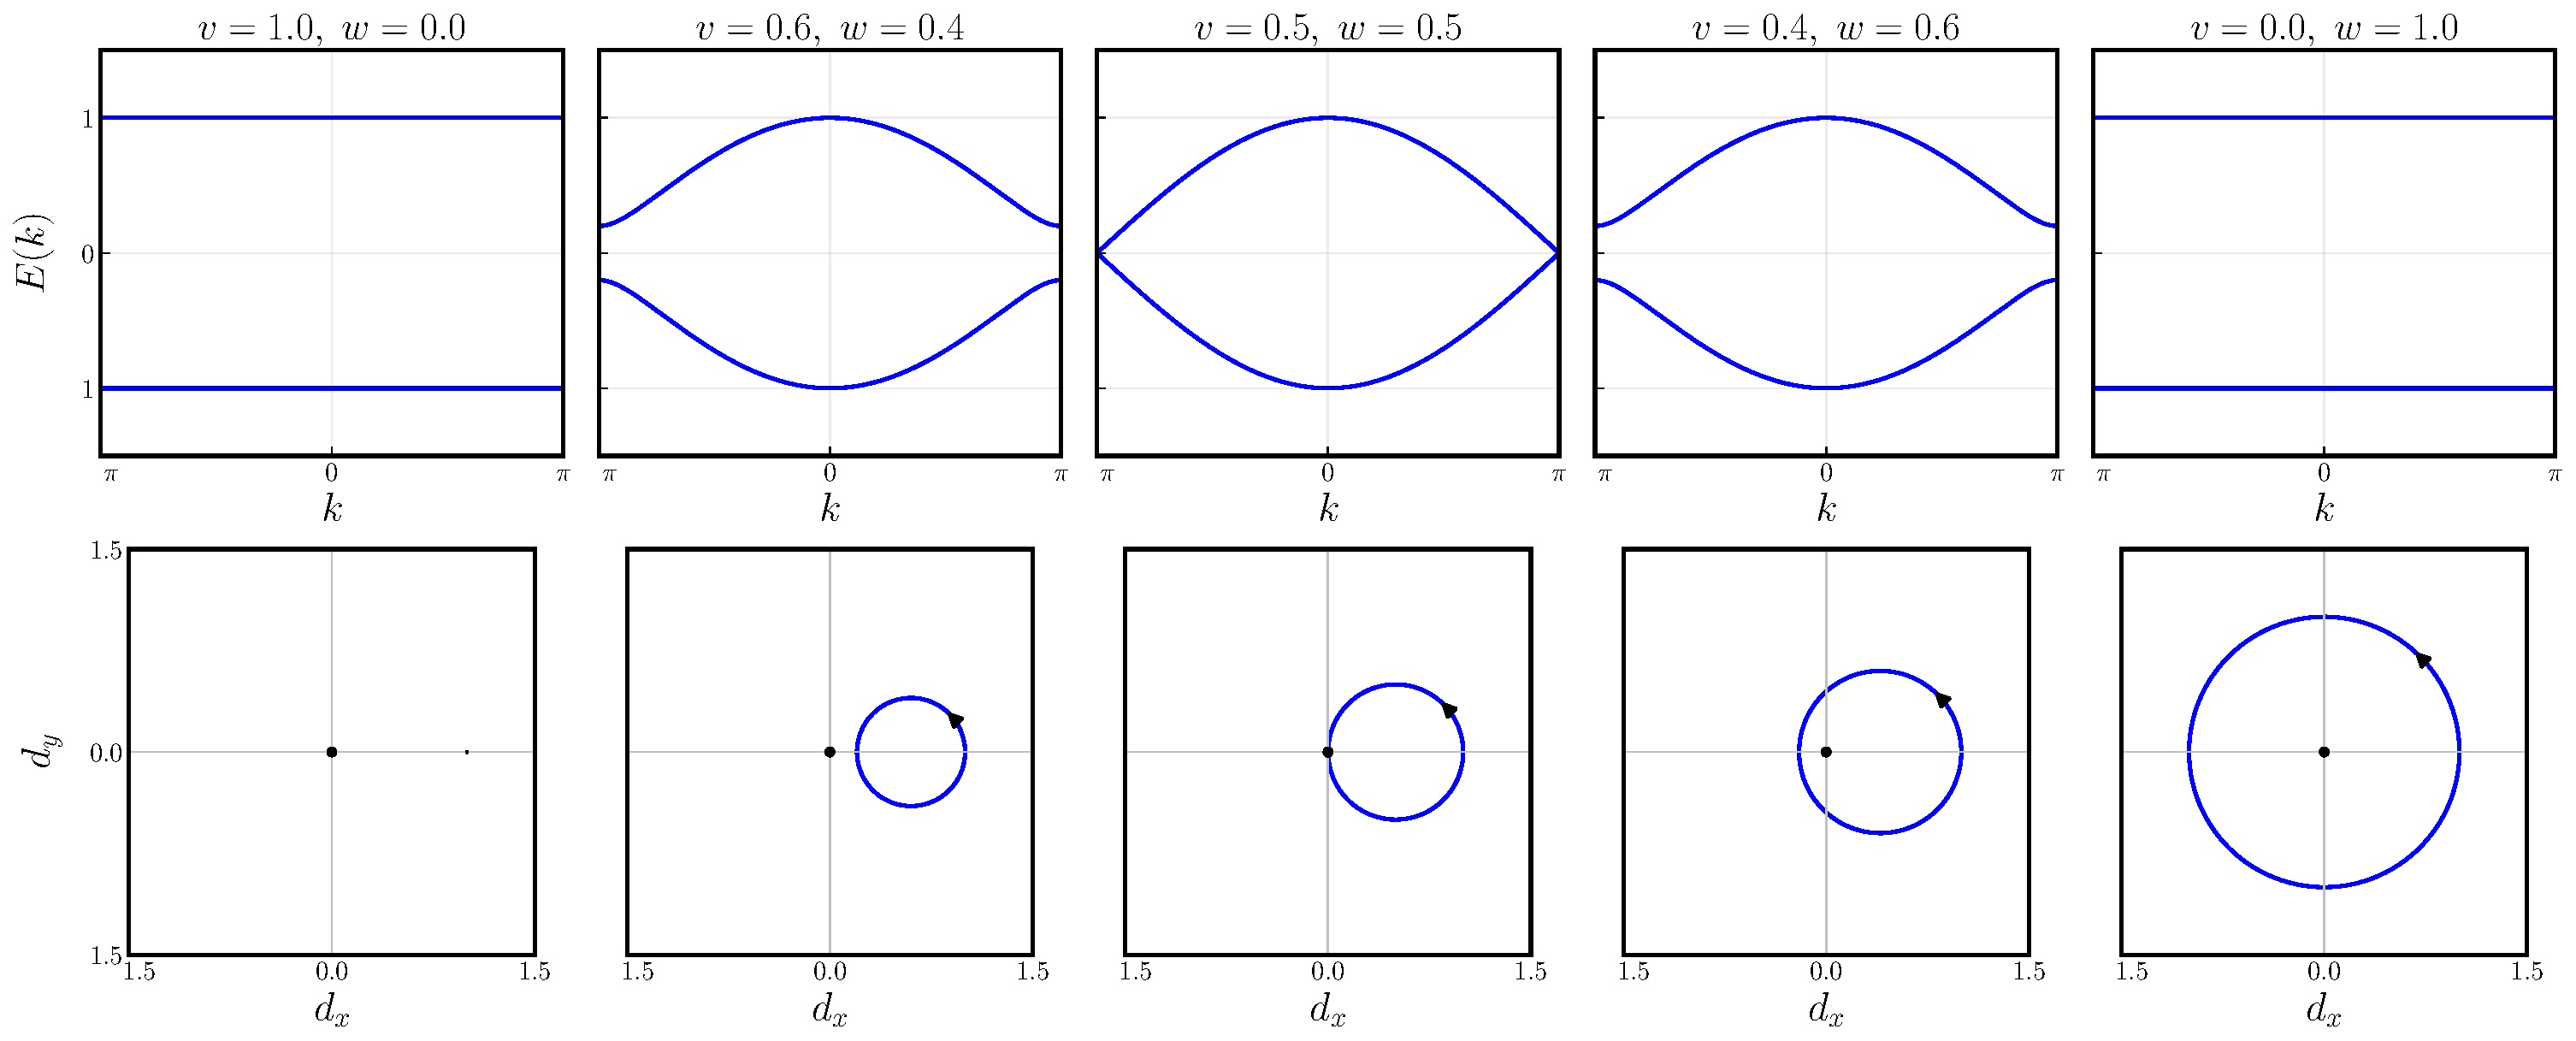
\includegraphics[width=\linewidth]{Figures/ssh_bands_winding.pdf}
\caption{
Energy dispersion (top row) and corresponding winding trajectories of $\mathbf{d}(k)$ in the $(d_x,d_y)$ plane (bottom row) for the SSH model with different intracell $v$ and intercell $w$ hopping amplitudes.
The topology of the winding trajectory changes as the relative hopping amplitudes are varied.
At the critical point $v=w$, the bulk energy gap closes and the trajectory passes through the origin, marking the topological phase transition.
}
\label{fig:bands_winding}
\end{figure}
\FloatBarrier

\subsection{Chiral Symmetry}
In addition to translational symmetry, the SSH model possesses an important internal symmetry known as \textit{chiral symmetry} \cite{asboth2015}. This symmetry plays a central role in determining the topological properties of the model and is responsible for the existence and protection of zero-energy edge states. Unlike translational symmetry, which is associated with the periodicity of the lattice, chiral symmetry relates the two sublattices of the SSH chain and imposes a specific structure on the Hamiltonian.

Unlike ordinary unitary symmetries, which satisfy

\[
\hat{U}\hat{H}\hat{U}^{\dagger}=\hat{H},
\]

chiral symmetry is characterized by an additional minus sign,

\[
\hat{\Gamma}\hat{H}\hat{\Gamma}^{\dagger}=-\hat{H}.
\]

This distinction has profound consequences for the spectrum of the Hamiltonian. While ordinary symmetries partition the Hilbert space into independent symmetry sectors, chiral symmetry instead relates eigenstates with positive and negative energies, leading to a spectrum that is symmetric about zero energy.
\vspace{1em}

\paragraph{Definition:}

A Hamiltonian is said to possess chiral symmetry if there exists a unitary operator
$\hat{\Gamma}$ satisfying

\begin{equation}
\hat{\Gamma}\hat{H}\hat{\Gamma}^{\dagger}
=
-\hat{H}.
\label{eq:chiral_definition}
\end{equation}

Since the chiral operator is unitary,

\begin{equation*}
\hat{\Gamma}^{\dagger}\hat{\Gamma}
=
\hat{\Gamma}\hat{\Gamma}^{\dagger}
=
I,
\end{equation*}

\cref{eq:chiral_definition} may be written equivalently as

\begin{equation*}
    \{ \hat{\Gamma},\hat{H}\} = 0
\end{equation*}

where

\[
\{A,B\}=AB+BA
\]

denotes the anticommutator.


\paragraph{Conditions:}

For the SSH model, the chiral operator satisfies the following properties.

\begin{enumerate}

\item
The operator $\hat{\Gamma}$ is unitary and Hermitian,

\begin{equation*}
\hat{\Gamma}^{\dagger}
=
\hat{\Gamma},
\qquad
\hat{\Gamma}^{2}
=
I.
\end{equation*}
The requirement that the chiral operator be both unitary and Hermitian ensures that
\(\Gamma^2=I\). If this condition were not satisfied, the operator
\(\Gamma^2\) would itself generate an ordinary unitary symmetry of the Hamiltonian.
Thus, imposing \(\Gamma^2=I\) guarantees that chiral symmetry represents a distinct
symmetry class rather than an ordinary unitary symmetry.

\item
The operator acts locally within each unit cell and distinguishes the two
sublattices through its eigenvalues. Since the chiral operator is Hermitian and
satisfies

\[
\Gamma^2=I,
\]

its eigenvalues are restricted to \(\pm1\). Choosing the sublattice basis to
coincide with the eigenbasis of the chiral operator, the basis states satisfy

\[
\Gamma|A\rangle=|A\rangle,
\qquad
\Gamma|B\rangle=-|B\rangle.
\]

Thus, the $A$ and $B$ sublattices correspond to the positive- and
negative-chirality eigenspaces, respectively. In this basis the chiral operator
is represented by

\[
\Gamma=\sigma_z.
\]

To verify that $\Gamma= \sigma_z$ indeed generates chiral symmetry, consider the momentum-space Hamiltonian of the SSH model,

\begin{equation}
H(k)=d_x(k)\sigma_x+d_y(k)\sigma_y .
\end{equation}

Since $\sigma_z$ is Hermitian and unitary,
\[
\sigma_z^\dagger=\sigma_z,\qquad \sigma_z^2=I,
\]
we evaluate

\begin{align}
\sigma_z H(k)\sigma_z
&=\sigma_z\left[d_x(k)\sigma_x+d_y(k)\sigma_y\right]\sigma_z \\
&=d_x(k)\sigma_z\sigma_x\sigma_z
+d_y(k)\sigma_z\sigma_y\sigma_z.
\end{align}

Using the anticommutation relations of the Pauli matrices,

\[
\{\sigma_i,\sigma_j\}=2\delta_{ij}I,
\]

one finds

\[
\sigma_z\sigma_x\sigma_z=-\sigma_x,\qquad
\sigma_z\sigma_y\sigma_z=-\sigma_y.
\]

then we obtain

\begin{align}
\sigma_z H(k)\sigma_z
&=-d_x(k)\sigma_x-d_y(k)\sigma_y \\
&=-H(k).
\end{align}

Hence,

\begin{equation}
\sigma_z H(k)\sigma_z^\dagger=-H(k),
\end{equation}

which is precisely the defining condition for chiral symmetry. Equivalently,

\begin{equation}
\{\sigma_z,H(k)\}=0.
\end{equation}

The above result is possible because the SSH Hamiltonian contains only the
$\sigma_x$ and $\sigma_y$ Pauli matrices,

\[
H(k)=d_x(k)\sigma_x+d_y(k)\sigma_y,
\]

with no $\sigma_z$ component, i.e.,

\[
d_z(k)=0.
\]

Consequently, the vector
\[
\mathbf d(k)=\left(d_x(k),\,d_y(k),\,0\right)
\]
is constrained to lie entirely in the $d_x$--$d_y$ plane. This geometric
constraint is essential for defining the winding number, which classifies the
topological phases of the SSH model. Physically, the absence of a $\sigma_z$
term reflects the bipartite nature of the lattice: hopping occurs only between different sublattices, while no terms couple sites within the same sublattice or produce an on-site energy difference between them.

\item
Chiral symmetry is robust under variations of the hopping amplitudes, provided that
the bipartite nature of the lattice is preserved. In practice, this means that the
intracell and intercell hopping amplitudes may vary from bond to bond due to
disorder, while the Hamiltonian continues to satisfy

\[
\hat{\Gamma}\hat{H}\hat{\Gamma}^{\dagger}
=
-\hat{H},
\]

as long as hopping occurs only between opposite sublattices. The chiral symmetry
operator itself remains independent of these local variations in the hopping
parameters.

\end{enumerate}

The localization of zero-energy states on a single sublattice plays a fundamental
role in the SSH model. In the topological phase, these zero-energy states appear as
edge states localized at opposite ends of a finite chain. Their existence is protected
by chiral symmetry, and they remain pinned at zero energy as long as the symmetry
and the bulk energy gap are preserved.


\subsubsection{Why Chiral Symmetry Implies an Off-Diagonal Hamiltonian}

In the previous section, the SSH Hamiltonian was shown to satisfy the chiral symmetry condition

\[
    \{\Gamma, H \} = 0.
\]

Throughout the literature, Hamiltonians possessing chiral symmetry are commonly written in the block off-diagonal form

\[
    H= \begin{pmatrix}
        0 & q \\
        q^{\dagger} & 0
    \end{pmatrix}.
\]

This form is not an arbitrary choice of notation. Rather, it follows directly from the algebraic properties of the chiral symmetry operator. In this section, we show that every Hermitian Hamiltonian possessing chiral symmetry can always be represented in this form by choosing the eigenbasis of the chiral operator.

\paragraph{Spectral properties of the chiral operator}:

The chiral operator satisfies

\[
    \Gamma^{\dagger} = \Gamma,
\]

and 

\[
    \Gamma^2 = I
\]

Since $\Gamma$ is Hermitian, the Spectral Theorem guarantees that every Hermitian operator can be diagonalized by a unitary transformation. Consequently, there exists a unitary matrix $U$ such that,
\[  U^{\dagger}\Gamma U = D,\]
where $D$ is diagonal matrix containing the eigenvalues of $\Gamma$.

The columns of $U$ are orthonormal eigenvectors of $\Gamma$. Expressing all vectors and operators in this basis is referred to as choosing the eigenbasis of the chiral operator. Since a change of basis does not alter the physical content of the theory, we are always free to work in this representation.

\paragraph{What does the diagonal matrix D look like?} 
Suppose \[ \Gamma |u\rangle = \lambda|u\rangle.\]

Applying $\Gamma$ once more,
\[
    \Gamma^2|u\rangle = \lambda^2|u\rangle
\]
Since
    \[
        \Gamma^2 = I
    \]
it follows that
\[
    \lambda^2 =1
\]
Hence
\[
    \lambda = \pm1.
\]
Therefore
\[
    D = \begin{pmatrix}
        I & 0\\
        0 & -I
    \end{pmatrix}
\]
where the basis has been ordered such that all eigenvectors with eigenvalue $+1$ are placed before those with eigenvalue $-1$. The identity matrices $I$ denote the identity operator acting within the corresponding eigenspaces.


For the SSH model, the internal Hilbert space is two-dimensional, with one eigenvector corresponding to each eigenvalue. Consequently,

\[
D=\sigma_z=
\begin{pmatrix}
1&0\\
0&-1
\end{pmatrix}.
\]

Thus, the familiar representation of the chiral operator in the SSH model is simply the two-dimensional realization of the general diagonal form derived above.

Having established the form of the chiral operator in its eigenbasis, we now consider the most general Hermitian Hamiltonian acting on the same Hilbert space. Since the Hilbert space has been decomposed into two orthogonal eigenspaces of $\Gamma$, every linear operator acting on this space admits a corresponding block-matrix representation. In this basis, the Hamiltonian may be written as

\[
H=
\begin{pmatrix}
A&B\\
C&D
\end{pmatrix},
\]

where the matrices $A$ and $D$ describe transitions within the positive-
and negative-chirality subspaces, respectively, while $B$ and $C$
describe transitions between the two subspaces.

The defining property of chiral symmetry is that the Hamiltonian
anticommutes with the chiral operator,


\[
\{\Gamma,H\}=0.
\]

Using the diagonal representation

\[
\Gamma=
\begin{pmatrix}
I&0\\
0&-I
\end{pmatrix},
\]

we first evaluate the product $\Gamma H$,

\[
\Gamma H
=
\begin{pmatrix}
I&0\\
0&-I
\end{pmatrix}
\begin{pmatrix}
A&B\\
C&D
\end{pmatrix}
=
\begin{pmatrix}
A&B\\
-C&-D
\end{pmatrix}.
\]

Similarly,

\[
H\Gamma
=
\begin{pmatrix}
A&B\\
C&D
\end{pmatrix}
\begin{pmatrix}
I&0\\
0&-I
\end{pmatrix}
=
\begin{pmatrix}
A&-B\\
C&-D
\end{pmatrix}.
\]

Adding the two matrices gives

\[
\Gamma H+H\Gamma
=
\begin{pmatrix}
2A&0\\
0&-2D
\end{pmatrix}.
\]

Since chiral symmetry requires

\[
\Gamma H+H\Gamma=0,
\]

it immediately follows that

\[
A=0,
\qquad
D=0.
\]

Therefore, every Hamiltonian possessing chiral symmetry must have the form

\[
H=
\begin{pmatrix}
0&B\\
C&0
\end{pmatrix}.
\]

Since the Hamiltonian represents a physical observable, it must also be
Hermitian,

\[
H^\dagger=H.
\]

Taking the Hermitian conjugate of the above matrix,

\[
H^\dagger
=
\begin{pmatrix}
0&C^\dagger\\
B^\dagger&0
\end{pmatrix}.
\]

Comparing this expression with

\[
H=
\begin{pmatrix}
0&B\\
C&0
\end{pmatrix},
\]

gives

\[
C=B^\dagger.
\]

Defining

\[
q\equiv B,
\]

the Hamiltonian finally assumes the form

\[
H=
\begin{pmatrix}
0&q\\
q^\dagger&0
\end{pmatrix}.
\]
This result is equivalent to the projection operator formulation discussed in the following subsection.

Hence, the block off-diagonal structure of the Hamiltonian is not an
additional assumption but follows directly from the existence of chiral
symmetry together with the Hermiticity of the Hamiltonian.

\paragraph{Physical Interpretation}

The matrices $A$ and $D$ describe transitions between states having the same
chirality, while $B$ and $C$ describe transitions between states of opposite
chirality. The anticommutation relation forbids the former, forcing the
diagonal blocks of the Hamiltonian to vanish. Consequently, a
chiral-symmetric Hamiltonian only couples states belonging to opposite
chiral sectors.

For the SSH model, these two chiral sectors correspond to the $A$ and $B$
sublattices. Since hopping occurs only between opposite sublattices and
never within the same sublattice, the Hamiltonian naturally possesses the
block off-diagonal structure derived above.

\paragraph{Remark}

The proof presented above is completely general and does not rely on any
specific property of the SSH model. Any Hermitian Hamiltonian satisfying

\[
\{\Gamma,H\}=0
\]

can always be transformed into the block off-diagonal form by working in the
eigenbasis of the chiral operator. The SSH Hamiltonian is therefore a
particular realization of this general mathematical result.



\subsubsection{Consequences of Chiral Symmetry}
The anticommutation relation between the Hamiltonian and the chiral operator,

\[
\{\Gamma,H\}=0,
\]

imposes several important constraints on the spectrum and eigenstates of the SSH model. These consequences are discussed below.

\paragraph{Sublattice Symmetry}

An alternative and often useful characterization of chiral symmetry is obtained
through projection operators onto the two sublattices. Defining

\begin{equation}
\hat P_A=\frac12(I+\hat\Gamma),
\qquad
\hat P_B=\frac12(I-\hat\Gamma),
\end{equation}

the operators satisfy

\[
\hat P_A+\hat P_B=I,
\qquad
\hat P_A\hat P_B=0,
\]

and project an arbitrary state onto the \(A\)- and \(B\)-sublattice
subspaces, respectively.

Using the anticommutation relation

\[
\{\hat\Gamma,\hat H\}=0,
\]

one finds

\[
\hat P_A\hat H\hat P_A=0,
\qquad
\hat P_B\hat H\hat P_B=0.
\]

Thus, the Hamiltonian possesses no matrix elements connecting sites within the
same sublattice. Equivalently, the only non-vanishing matrix elements are those
between opposite sublattices,

\[
\hat H
=
\hat P_A\hat H\hat P_B
+
\hat P_B\hat H\hat P_A.
\]

This projection-operator formulation is completely equivalent to the block
off-diagonal representation derived in the previous subsection and provides a
basis-independent description of sublattice (chiral) symmetry.

\paragraph{Symmetric Energy Spectrum}

Suppose that \(|\psi_n\rangle\) is an eigenstate of the Hamiltonian,

\begin{equation}
\hat{H}|\psi_n\rangle
=
E_n|\psi_n\rangle.
\end{equation}

Multiplying from the left by the chiral operator gives

\begin{align*}
\hat{\Gamma}\hat{H}|\psi_n\rangle
&=
E_n\hat{\Gamma}|\psi_n\rangle.
\end{align*}

Using the anticommutation relation,

\[
\hat{\Gamma}\hat{H}
=
-\hat{H}\hat{\Gamma},
\]

we obtain

\begin{align*}
-\hat{H}\hat{\Gamma}|\psi_n\rangle
&=
E_n\hat{\Gamma}|\psi_n\rangle,
\end{align*}

or equivalently,

\begin{equation}
\hat{H}\left(\hat{\Gamma}|\psi_n\rangle\right)
=
-E_n
\left(\hat{\Gamma}|\psi_n\rangle\right).
\end{equation}

Hence, if \(E_n\) is an eigenvalue of the Hamiltonian, then \(-E_n\) is also an eigenvalue. Chiral symmetry therefore guarantees that the energy spectrum is symmetric about zero energy.


\paragraph{Equal Support on Both Sublattices}

Consider an eigenstate with non-zero energy,

\[
|\psi_n\rangle
=
\begin{pmatrix}
a\\
b
\end{pmatrix},
\]

where \(a\) and \(b\) denote the amplitudes on the two sublattices.

Since the chiral operator is represented by

\[
\hat{\Gamma}
=
\sigma_z
=
\begin{pmatrix}
1&0\\
0&-1
\end{pmatrix},
\]

we obtain

\[
\hat{\Gamma}
|\psi_n\rangle
=
\begin{pmatrix}
a\\
-b
\end{pmatrix}.
\]

Because eigenstates corresponding to different eigenvalues are orthogonal,

\begin{equation*}
\langle\psi_n|
\hat{\Gamma}
|\psi_n\rangle
=
0.
\end{equation*}

Substituting the above expression,

\begin{align*}
0
&=
(a^*,b^*)
\begin{pmatrix}
a\\
-b
\end{pmatrix}
\\
&=
|a|^2-|b|^2.
\end{align*}

Therefore,

\begin{equation*}
|a|^2
=
|b|^2.
\end{equation*}

Thus, every non-zero-energy eigenstate has equal probability on the two sublattices.

\paragraph{Zero-Energy Eigenstates}

The above argument applies only to states with non-zero energy. For a zero-energy eigenstate,

\[
\hat{H}|\psi_0\rangle=0,
\]

there is no requirement that the state possesses equal support on both sublattices. Instead, the eigenstate may be chosen to reside entirely on a single sublattice.

This property plays a fundamental role in the SSH model, as the topological edge states appearing in the non-trivial phase are zero-energy eigenstates localized on opposite ends of the chain and occupy only one of the two sublattices.

\subsection{Winding Number}

The energy dispersion derived in the previous section shows that the SSH model possesses two insulating phases separated by a gap-closing point at \(v=w\). Although both phases are characterized by a finite bulk band gap, they cannot be distinguished solely from the energy spectrum. A quantity that remains invariant under continuous deformations of the Hamiltonian, provided the energy gap remains open, is therefore required to classify these phases. Such a quantity is known as a \textit{topological invariant}. For the SSH model, the relevant topological invariant is the winding number.~\cite{asboth2015,hasan2010,qi2011}

From \cref{eq:dvector}, the momentum-space Hamiltonian can be written as

\begin{equation*}
H(k)=\mathbf{d}(k)\cdot\boldsymbol{\sigma},
\end{equation*}

where

\begin{equation*}
\mathbf{d}(k)=
\left(
d_x(k),
d_y(k),
0
\right),
\end{equation*}

with

\begin{align*}
d_x(k)&=v+w\cos k,\\
d_y(k)&=w\sin k.
\end{align*}

Since chiral symmetry forbids the presence of a \(\sigma_z\) term, the vector
\(\mathbf d(k)\) is constrained to lie entirely in the \(d_x\)-\(d_y\) plane. As the crystal momentum \(k\) varies continuously over the first Brillouin zone,

\[
-\pi\leq k\leq\pi,
\]

the endpoint of the vector \(\mathbf d(k)\) traces a closed trajectory in this plane. The topology of this trajectory provides the basis for defining the winding number.

To characterize the topology of the curve, it is convenient to introduce the normalized vector

\begin{equation*}
\hat{\mathbf d}(k)
=
\frac{\mathbf d(k)}
{|\mathbf d(k)|},
\end{equation*}

which lies on the unit circle. The winding number counts the number of times the vector
\(\hat{\mathbf d}(k)\) winds around the origin as \(k\) traverses the Brillouin zone once. It is given by

\begin{equation}
\nu
=
\frac{1}{2\pi}
\int_{-\pi}^{\pi}
\left(
\hat{\mathbf d}
\times
\frac{d\hat{\mathbf d}}{dk}
\right)_z
dk.
\label{eq:winding}
\end{equation}

The subscript \(z\) denotes the component perpendicular to the \(d_x\)-\(d_y\) plane. Since the trajectory is confined to this plane, the cross product points entirely along the \(z\)-direction, and the integral measures the total angular change of the vector during one complete traversal of the Brillouin zone.

An equivalent and often more convenient formulation is obtained by introducing the complex function

\begin{equation*}
q(k)
=
d_x(k)-id_y(k)
=
v+we^{-ik}.
\end{equation*}

Using this definition, the bulk Hamiltonian may be written as

\begin{equation*}
H(k)=
\begin{pmatrix}
0&q(k)\\
q^{\dagger}(k)&0
\end{pmatrix},
\end{equation*}

and the winding number takes the compact form

\begin{equation}
\nu
=
\frac{1}{2\pi i}
\int_{-\pi}^{\pi}
\frac{d}{dk}
\ln q(k)\,dk.
\label{eq:winding_complex}
\end{equation}

\cref{eq:winding_complex} measures the total change in the complex phase of
\(q(k)\) as the crystal momentum traverses the Brillouin zone. Since the phase can change only by integer multiples of \(2\pi\), the winding number is restricted to integer values and therefore represents a topological invariant.

The winding trajectories corresponding to different hopping amplitudes are shown in \cref{fig:bands_winding}. When the intracell hopping dominates (\(v>w\)), the trajectory does not enclose the origin, giving

\[
\nu=0,
\]

which corresponds to the trivial insulating phase. Conversely, when the intercell hopping exceeds the intracell hopping \(w>v\), the trajectory winds once around the origin, yielding

\[
\nu=1,
\]

which identifies the topological phase. At the critical point \(v=w\), the trajectory passes through the origin. Since the vector \(\mathbf d(k)\) vanishes at this point, the winding number becomes ill-defined, and the bulk energy gap simultaneously closes, signalling the topological phase transition.

The winding number is a topological invariant and therefore remains unchanged under any continuous deformation of the Hamiltonian that preserves both chiral symmetry and the bulk energy gap. Consequently, two phases with different winding numbers cannot be continuously transformed into one another without first closing the gap. The gap closure at \(v=w\) is therefore not merely a feature of the SSH model but a general characteristic of topological phase transitions in topological band systems \cite{hasan2010,qi2011}. When the gap closes, the normalized vector \(\mathbf d(k)\) becomes undefined at the gap-closing momentum, allowing the winding trajectory to pass through the origin and the winding number to change. After the gap reopens, the system may enter a topologically distinct phase characterized by a different winding number. This bulk topological distinction manifests itself in finite systems through the appearance of topologically protected edge states, discussed in the following section.

\subsection{Bulk--Boundary Correspondence}

The winding number introduced in the previous section is defined for the
infinite periodic SSH chain, where translational symmetry allows the
Hamiltonian to be expressed in momentum space. In contrast, the edge
states discussed in the following section appear only in finite systems
with open boundaries. The connection between these two seemingly
different descriptions is provided by the \emph{bulk--boundary
correspondence}.

The bulk--boundary correspondence states that the existence of
topologically protected boundary states is determined entirely by the
topological invariant of the bulk Hamiltonian as established in the literature \cite{asboth2015,hasan2010,qi2011}  . Consequently, the winding
number calculated for the infinite periodic system predicts the
appearance or absence of localized edge states in a finite chain.

For the SSH model, the correspondence is summarized as follows:

\[
\nu=
\begin{cases}
0, & \text{Trivial phase: no protected edge states,}\\[2mm]
1, & \text{Topological phase: one pair of zero-energy edge states.}
\end{cases}
\]

Thus, although the winding number is computed using the bulk momentum-space
Hamiltonian, its physical manifestation is observed through the
localized boundary states of a finite system. This remarkable connection
between bulk topology and boundary physics forms one of the fundamental
principles of topological condensed matter physics .

The numerical calculations presented in the following sections verify
this correspondence. In the topological phase $w>v$, the finite SSH
chain exhibits localized zero-energy edge states, whereas no such states
appear in the trivial phase $v>w$.
















\subsection{Finite SSH Chain with Open Boundary Conditions}

The bulk Hamiltonian derived in the previous sections assumes periodic boundary conditions, allowing the application of Bloch's theorem and the description of the system in momentum space. While this approach is convenient for studying the bulk band structure and topological invariants, it removes the physical boundaries of the lattice and therefore cannot describe edge states. To investigate the existence of localized boundary modes, it is necessary to consider a finite SSH chain with open boundary conditions.

For a finite chain consisting of \(N\) unit cells, the periodic connection between the last and the first unit cells is removed. Consequently, the intercell hopping between the \(N^{\text{th}}\) and the first unit cell is absent, and the Hamiltonian is written as

\begin{equation}
\hat{H}
=
v\sum_{m=1}^{N}
\left(
|m,B\rangle\langle m,A|
+\mathrm{h.c.}
\right)
+
w\sum_{m=1}^{N-1}
\left(
|m+1,A\rangle\langle m,B|
+\mathrm{h.c.}
\right).
\label{eq:finite_hamiltonian}
\end{equation}

Unlike the bulk Hamiltonian, \cref{eq:finite_hamiltonian} no longer possesses translational symmetry. As a result, Bloch's theorem cannot be applied, and the Hamiltonian must be represented directly as a finite matrix in the localized basis

\[
\{
|1,A\rangle,
|1,B\rangle,
|2,A\rangle,
|2,B\rangle,
\ldots,
|N,A\rangle,
|N,B\rangle
\}.
\]

For a chain containing \(N\) unit cells, the Hamiltonian is therefore represented by a \(2N\times2N\) Hermitian matrix of the form

\begin{equation}
H=
\begin{pmatrix}
0&v&0&0&\cdots&0\\
v&0&w&0&\cdots&0\\
0&w&0&v&\cdots&0\\
0&0&v&0&\ddots&\vdots\\
\vdots&\vdots&\vdots&\ddots&\ddots&w\\
0&0&0&\cdots&w&0
\end{pmatrix},
\label{eq:finite_matrix}
\end{equation}

where the alternating intracell and intercell hopping amplitudes appear as the off-diagonal matrix elements. Since the chain has open boundaries, the corner matrix elements are zero, distinguishing it from the periodic Hamiltonian.

The eigenvalues and eigenvectors of the finite Hamiltonian are obtained by solving the time-independent Schrödinger equation

\begin{equation}
H|\psi_n\rangle
=
E_n|\psi_n\rangle,
\end{equation}

where \(E_n\) denotes the energy eigenvalues and \(|\psi_n\rangle\) the corresponding eigenvectors. Owing to the finite size of the Hamiltonian matrix, the spectrum is obtained numerically by direct diagonalization. In the present work, the Hamiltonian was diagonalized using the \texttt{scipy.linalg.eigh()} routine, which computes the complete set of eigenvalues and orthonormal eigenvectors of a Hermitian matrix.

The numerical calculations were carried out for finite chains containing \(N=10\) and \(N=20\) unit cells, considering different values of the intracell and intercell hopping amplitudes. These calculations enable a direct comparison between the trivial phase (\(v>w\)) and the topological phase (\(w>v\)), and illustrate the emergence of localized edge states in the latter case.

The energy spectra obtained from the numerical diagonalization are presented in the following subsection. Subsequently, the corresponding eigenvectors are analysed to demonstrate the localization of the zero-energy states at the boundaries of the finite chain.

\subsubsection{Numerical Diagonalization}
\label{sec:numerical_diagonalization}
The finite SSH Hamiltonian was constructed numerically for chains containing \(N=10\) and \(N=20\) unit cells. Owing to the finite dimension of the Hamiltonian matrix, the complete energy spectrum and the corresponding eigenvectors were obtained by direct diagonalization using the \texttt{scipy.linalg.eigh()} routine, which computes the eigenvalues and orthonormal eigenvectors of a Hermitian matrix.

To investigate the topological phase transition, calculations were performed for four different hopping configurations,

\[
(v,w)=
(0.2,1.0),\;
(0.5,1.0),\;
(1.0,1.0),\;
(1.5,1.0),
\]

representing the topological phase (\(v<w\)), a point closer to the phase transition, the critical point (\(v=w\)), and the trivial insulating phase (\(v>w\)), respectively. For each parameter set, the complete energy spectrum was calculated and the eigenstate corresponding to the lowest positive-energy eigenvalue was analysed to investigate the spatial localization of the edge states.

\subsubsection{Energy Spectrum}
\label{sec:energy spectra}

The energy spectra obtained from the numerical diagonalization for finite chains containing \(N=10\) and \(N=20\) unit cells are shown in \cref{fig:spectrum10} and \cref{fig:spectrum20}. Each point represents an eigenvalue of the finite SSH Hamiltonian.

For \(v<w\), two eigenvalues appear very close to zero energy, corresponding to the topological edge states localized at opposite ends of the chain. As the hopping amplitudes approach the critical point \(v=w\), the bulk energy gap decreases continuously and closes at the transition. When \(v>w\), the bulk gap reopens and the near-zero-energy states disappear, indicating that the system has entered the trivial insulating phase.

Increasing the system size from \(N=10\) to \(N=20\) reduces the small energy splitting between the two edge states. This behaviour arises from the exponentially decreasing overlap between the states localized at opposite boundaries of the chain, causing their energies to approach zero with increasing chain length.

\begin{figure}[htbp]
    \centering
    \begin{subfigure}[b]{0.48\textwidth}
        \centering
        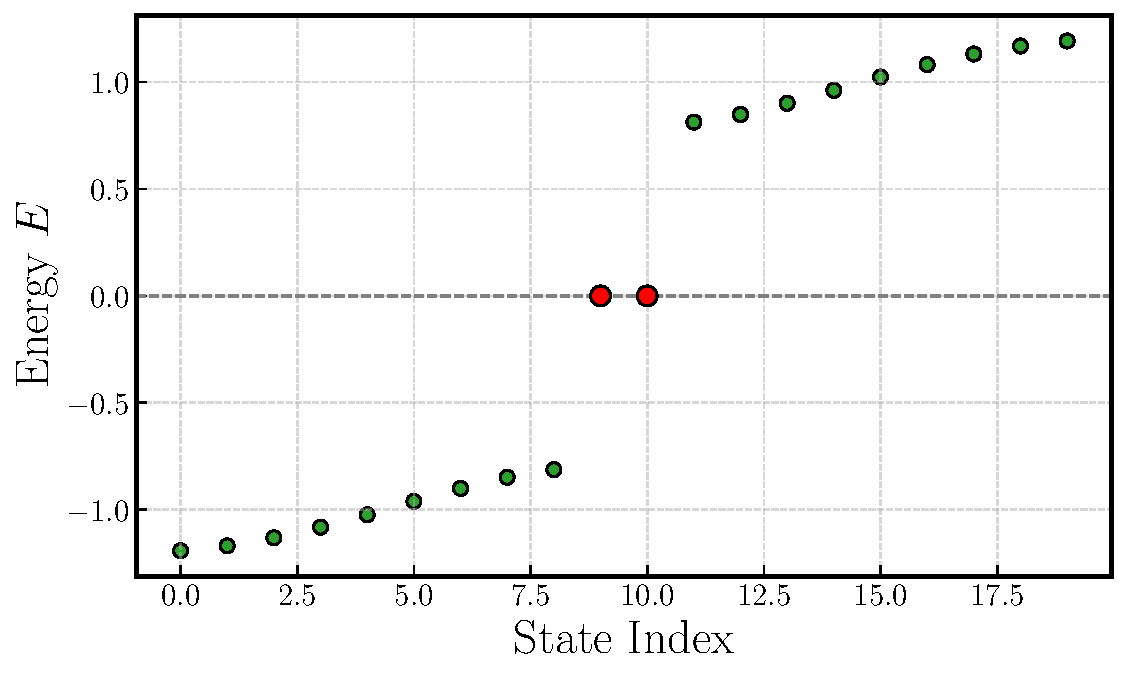
\includegraphics[width=\textwidth, max height=0.4\textheight, keepaspectratio]{Figures/spectrum_v=0.2_w=1.0_N=10.pdf}
        \caption{$v=0.2, w=1.0$}
        \label{fig:spec10_a}
    \end{subfigure}
    \hfill
    \begin{subfigure}[b]{0.48\textwidth}
        \centering
        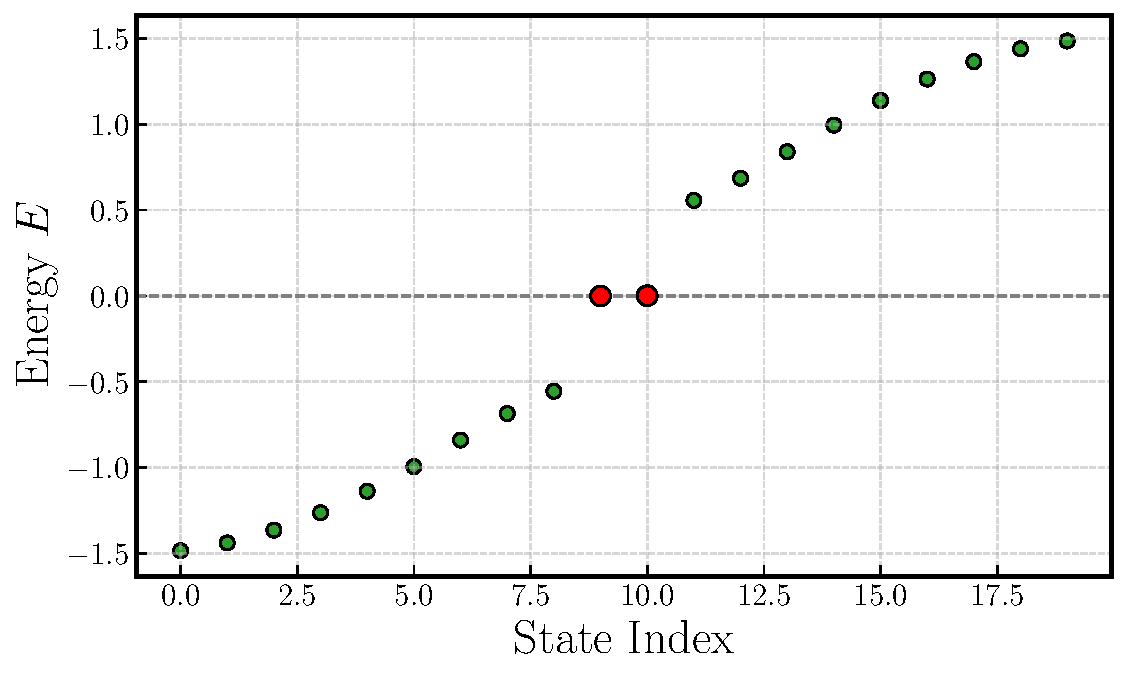
\includegraphics[width=\textwidth, max height=0.4\textheight, keepaspectratio]{Figures/spectrum_v=0.5_w=1.0_N=10.pdf}
        \caption{$v=0.5, w=1.0$}
        \label{fig:spec10_b}
    \end{subfigure}
    
    \vspace{0.4cm}
    
    \begin{subfigure}[b]{0.48\textwidth}
        \centering
        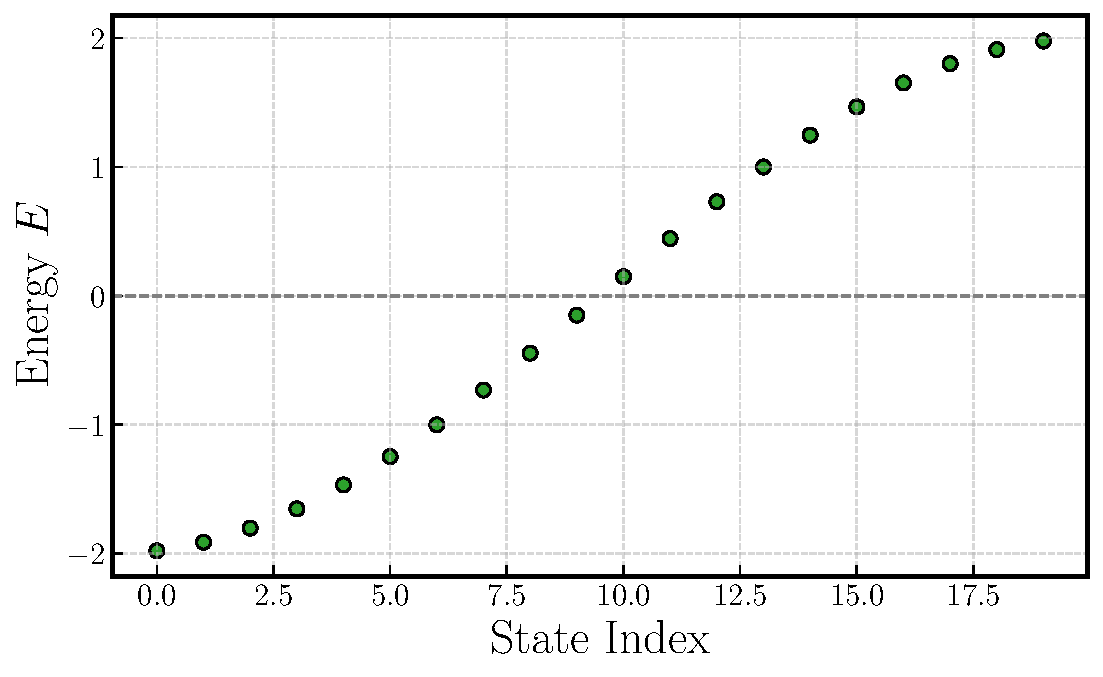
\includegraphics[width=\textwidth, max height=0.4\textheight, keepaspectratio]{Figures/spectrum_v=1.0_w=1.0_N=10.pdf}
        \caption{$v=1.0, w=1.0$}
        \label{fig:spec10_c}
    \end{subfigure}
    \hfill
    \begin{subfigure}[b]{0.48\textwidth}
        \centering
        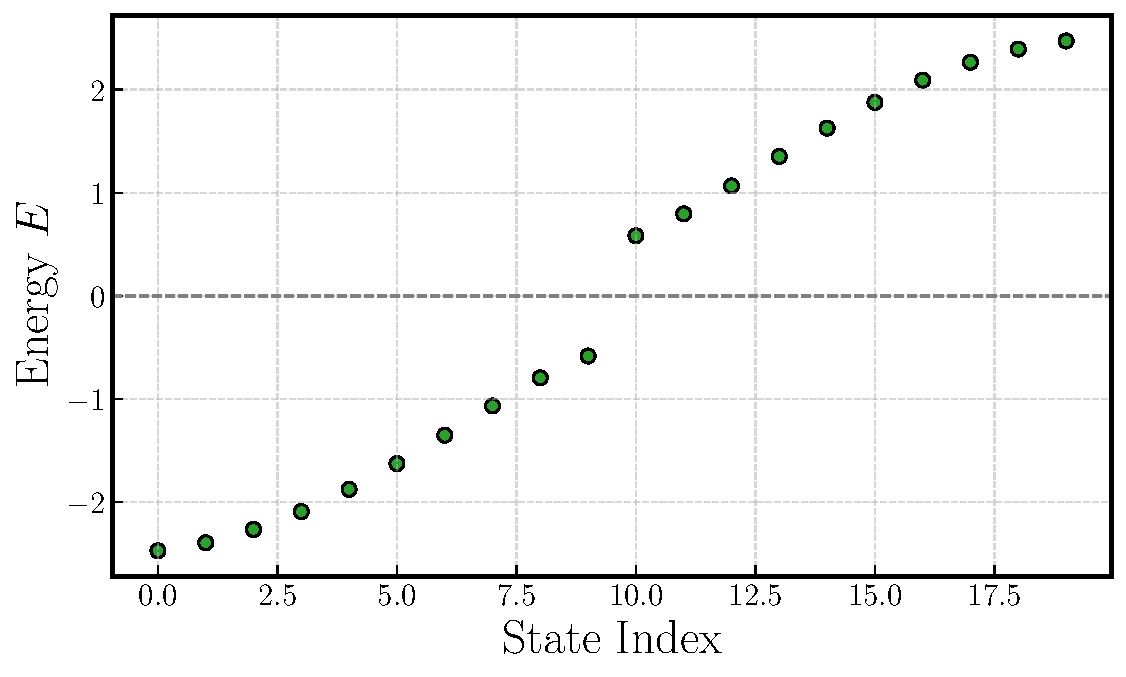
\includegraphics[width=\textwidth, max height=0.4\textheight, keepaspectratio]{Figures/spectrum_v=1.5_w=1.0_N=10.pdf}
        \caption{$v=1.5, w=1.0$}
        \label{fig:spec10_d}
    \end{subfigure}
    \caption{Energy spectra of the finite SSH chain containing $N=10$ unit cells. Two near-zero-energy states are observed in the topological phase ($v<w$), while they disappear in the trivial phase ($v>w$).}
    \label{fig:spectrum10}
\end{figure}

\begin{figure}[!htbp]
    \centering
    \begin{subfigure}[b]{0.48\textwidth}
        \centering
        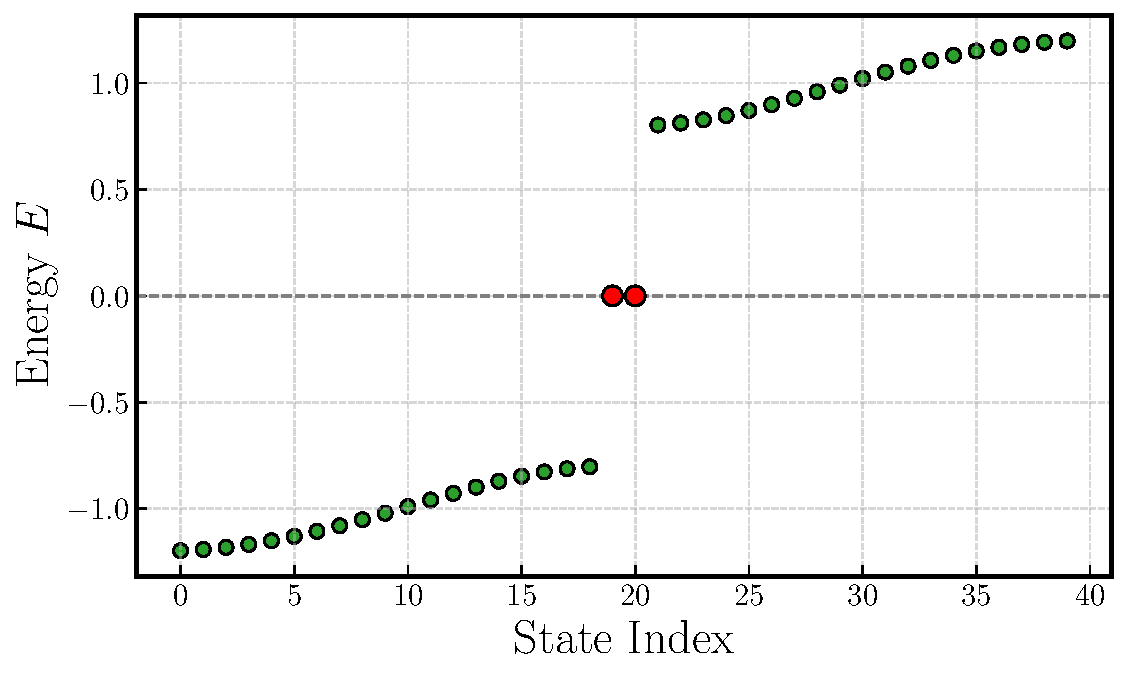
\includegraphics[width=\textwidth, max height=0.4\textheight, keepaspectratio]{Figures/spectrum_v=0.2_w=1.0_N=20.pdf}
        \caption{$v=0.2, w=1.0$}
    \end{subfigure}
    \hfill
    \begin{subfigure}[b]{0.48\textwidth}
        \centering
        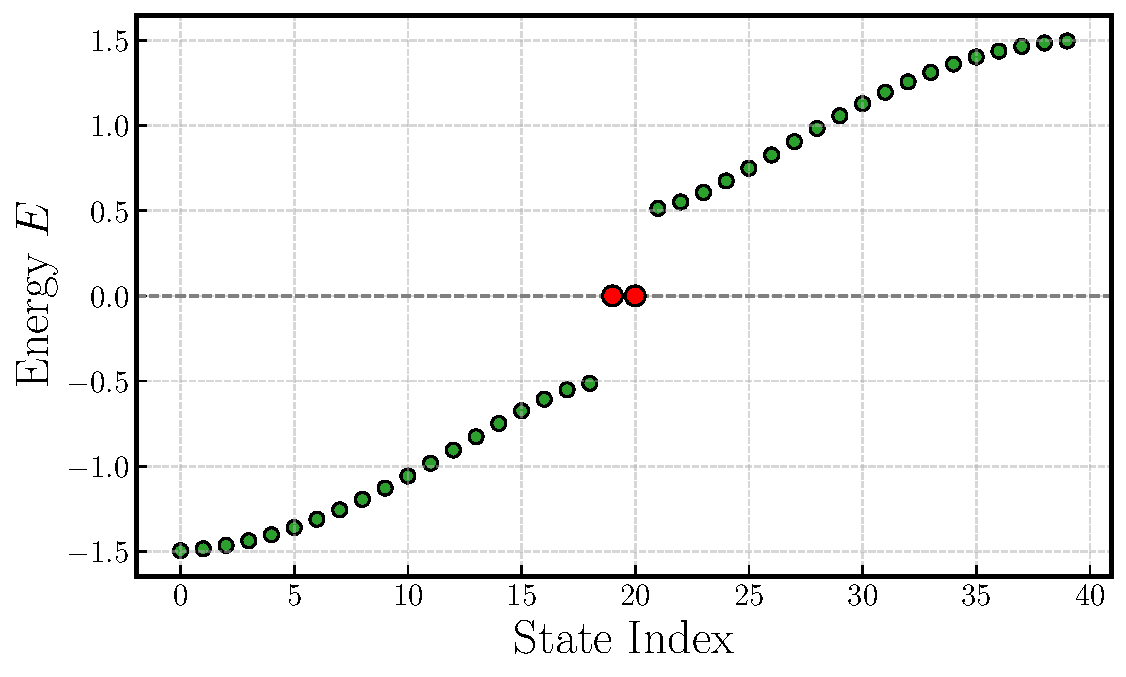
\includegraphics[width=\textwidth, max height=0.4\textheight, keepaspectratio]{Figures/spectrum_v=0.5_w=1.0_N=20.pdf}
        \caption{$v=0.5, w=1.0$}
    \end{subfigure}
    
    \vspace{0.4cm}
    
    \begin{subfigure}[b]{0.48\textwidth}
        \centering
        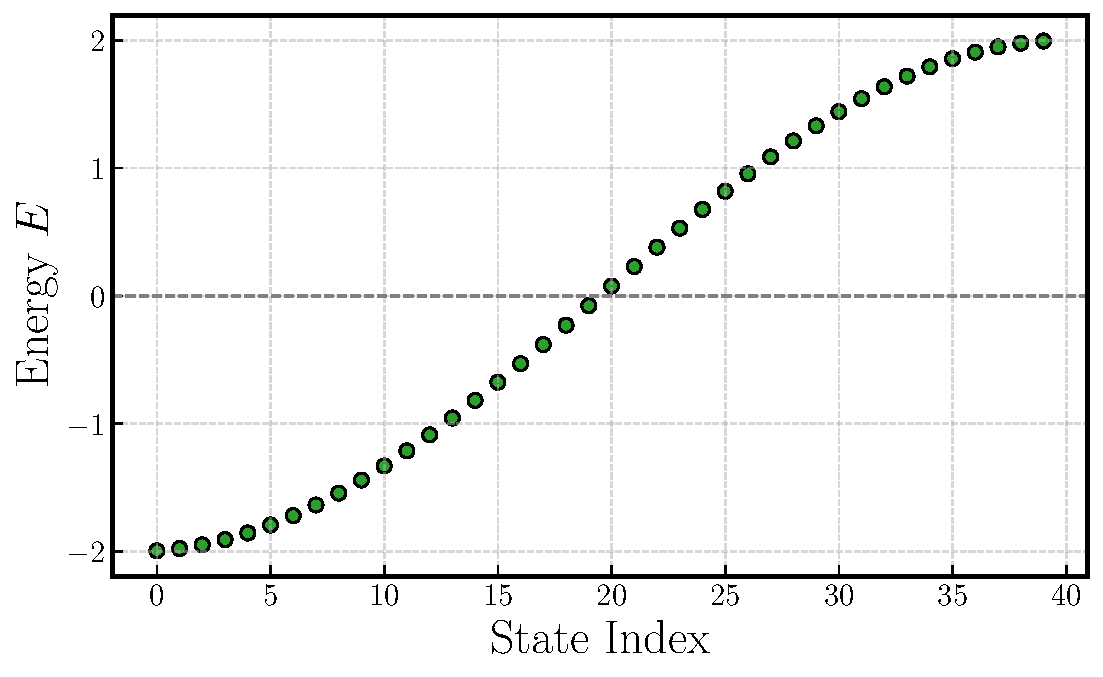
\includegraphics[width=\textwidth, max height=0.4\textheight, keepaspectratio]{Figures/spectrum_v=1.0_w=1.0_N=20.pdf}
        \caption{$v=1.0, w=1.0$}
    \end{subfigure}
    \hfill
    \begin{subfigure}[b]{0.48\textwidth}
        \centering
        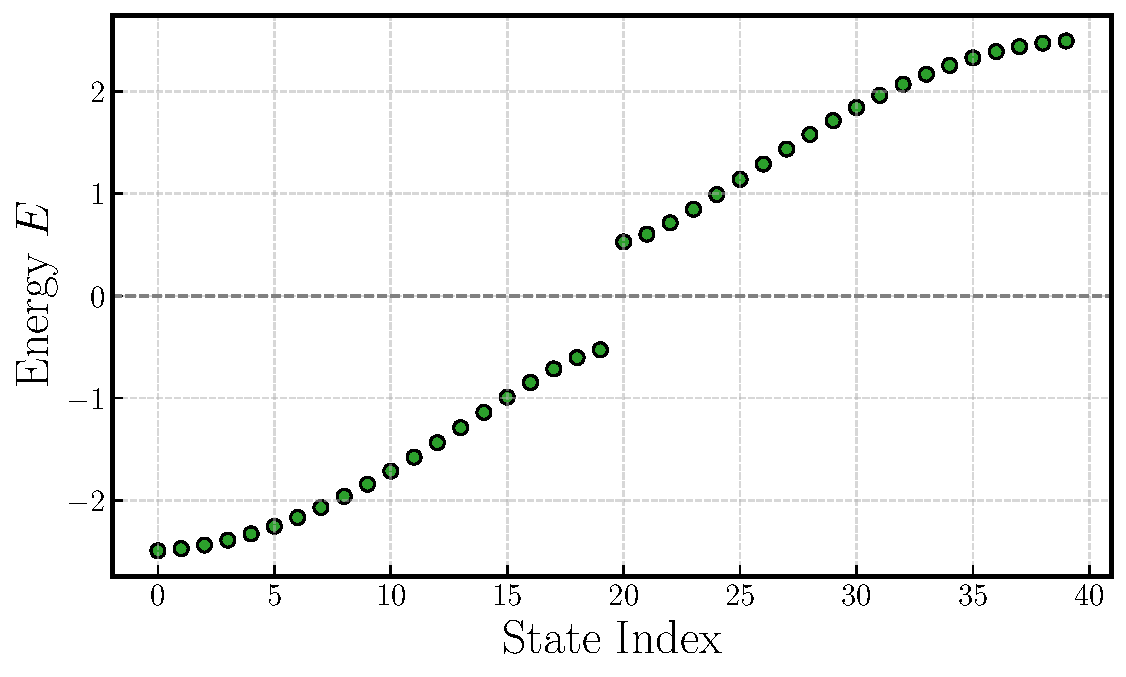
\includegraphics[width=\textwidth, max height=0.4\textheight, keepaspectratio]{Figures/spectrum_v=1.5_w=1.0_N=20.pdf}
        \caption{$v=1.5, w=1.0$}
    \end{subfigure}
    \caption{Energy spectra of the finite SSH chain containing \(N=20\) unit cells. Increasing the system size decreases the energy splitting between the edge states due to their exponentially weaker overlap.}
    \label{fig:spectrum20}
\end{figure}
\FloatBarrier
\subsubsection{Edge-State Probability Distribution}
\label{sec:edge_state_probability}

To identify the spatial localization of the topological edge states, the probability density associated with the eigenstate corresponding to the lowest positive-energy eigenvalue was calculated. For each unit cell, the probabilities on the two sublattices were obtained from the corresponding eigenvector according to

\begin{equation}
P_A(m)=|\psi_A(m)|^2,
\qquad
P_B(m)=|\psi_B(m)|^2,
\end{equation}

where \(m\) labels the unit cell.

The resulting probability distributions are shown in \cref{fig:prob10} and \cref{fig:prob20}. In the topological phase (\(v<w\)), the probability density is strongly localized near the boundaries of the chain, confirming the existence of topological edge states. As the system approaches the critical point (\(v=w\)), the localization length increases and the edge states extend further into the bulk. In contrast, for the trivial phase (\(v>w\)), the probability density is distributed throughout the lattice, indicating the absence of localized edge modes.

A comparison between \(N=10\) and \(N=20\) further shows that increasing the system size enhances the localization of the edge states by reducing their overlap, consistent with the behaviour observed in the energy spectra.


\begin{figure}[!htbp]
    \centering
    \begin{subfigure}[b]{0.48\textwidth}
        \centering
        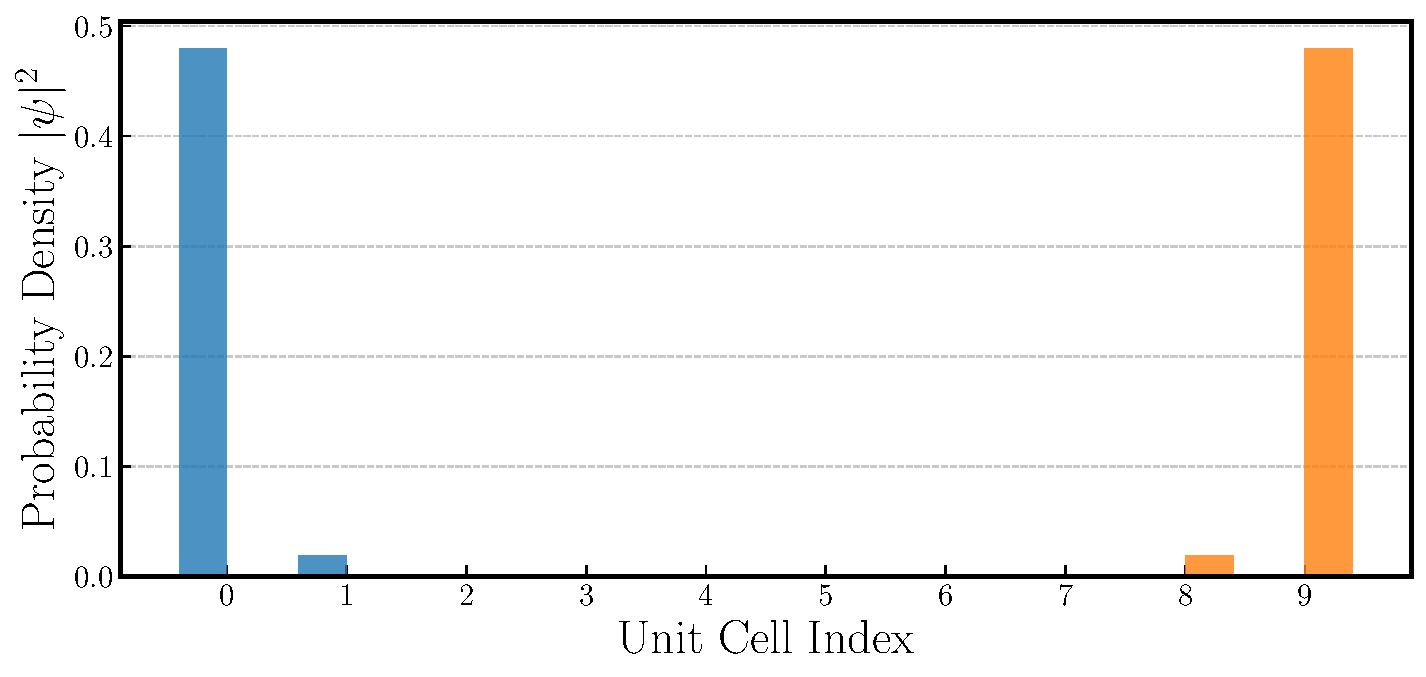
\includegraphics[width=\textwidth, max height=0.4\textheight, keepaspectratio]{Figures/probability_v=0.2_w=1.0_N=10.pdf}
        \caption{$v=0.2, w=1.0$}
    \end{subfigure}
    \hfill
    \begin{subfigure}[b]{0.48\textwidth}
        \centering
        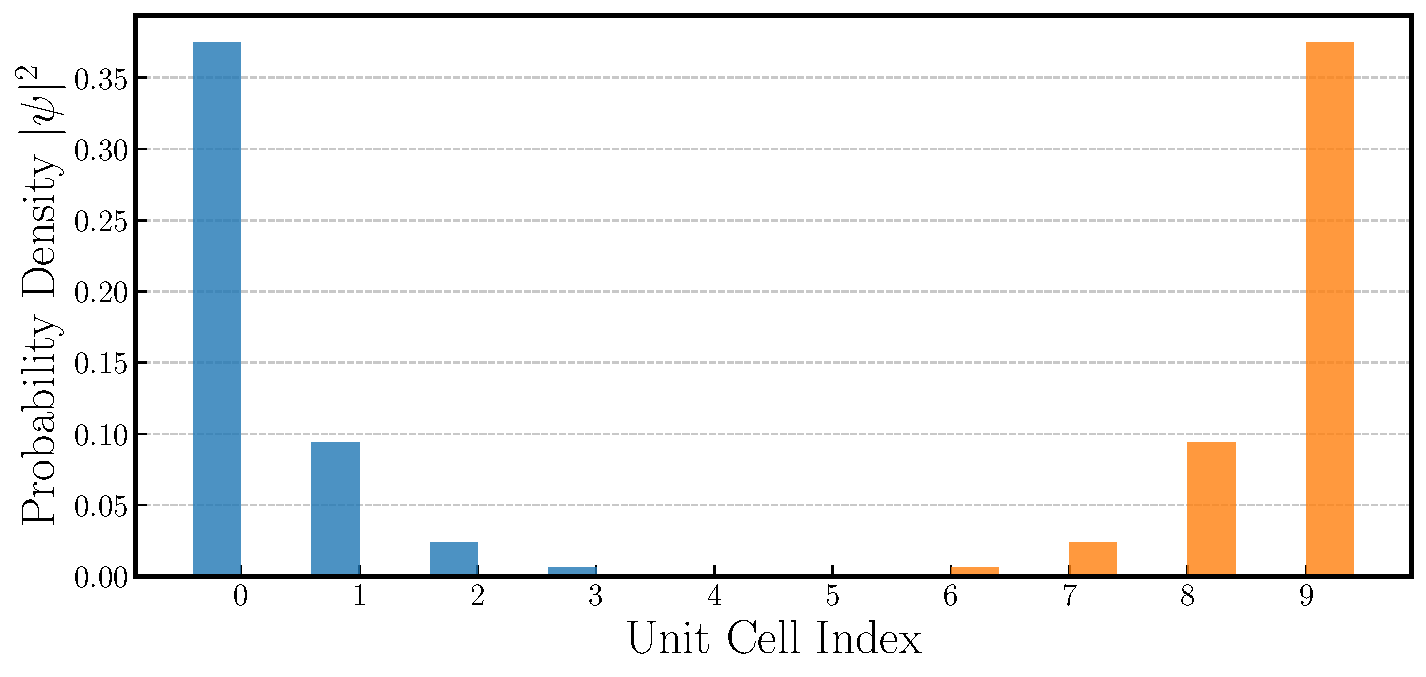
\includegraphics[width=\textwidth, max height=0.4\textheight, keepaspectratio]{Figures/probability_v=0.5_w=1.0_N=10.pdf}
        \caption{$v=0.5, w=1.0$}
    \end{subfigure}
    
    \vspace{0.4cm}
    
    \begin{subfigure}[b]{0.48\textwidth}
        \centering
        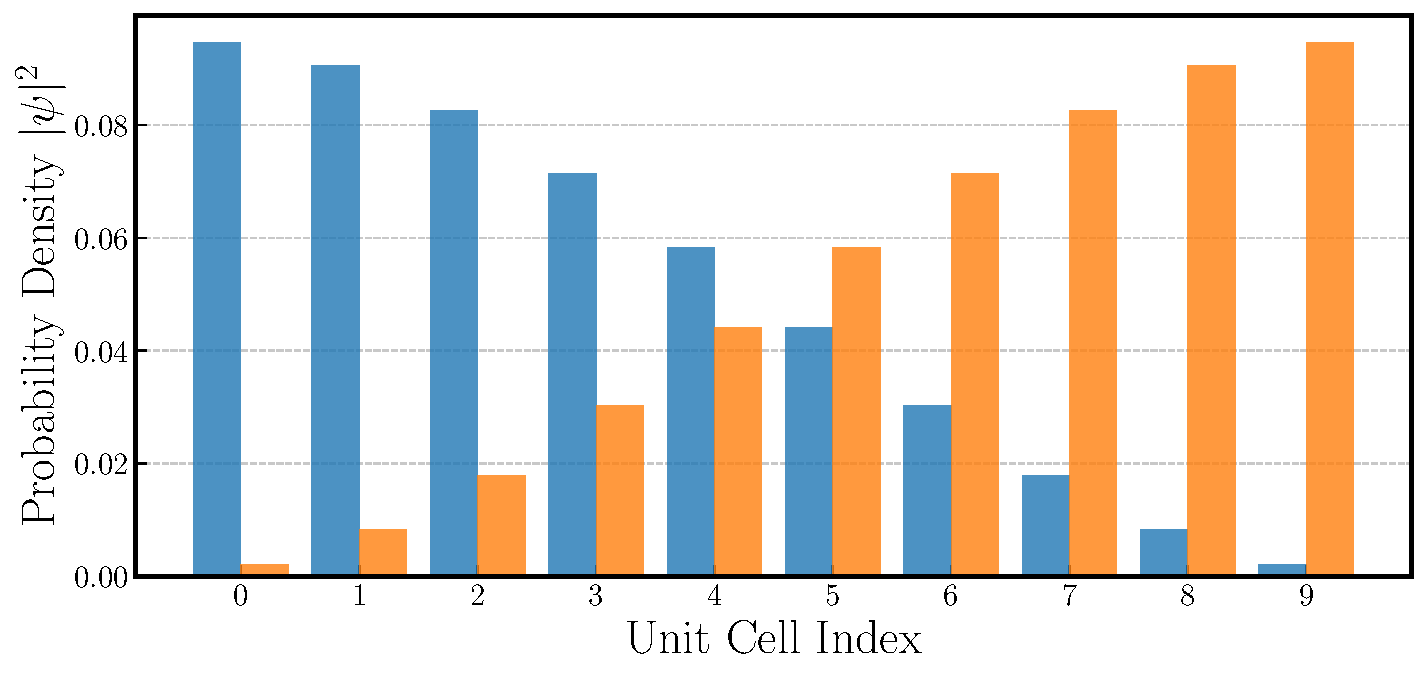
\includegraphics[width=\textwidth, max height=0.4\textheight, keepaspectratio]{Figures/probability_v=1.0_w=1.0_N=10.pdf}
        \caption{$v=1.0, w=1.0$}
    \end{subfigure}
    \hfill
    \begin{subfigure}[b]{0.48\textwidth}
        \centering
        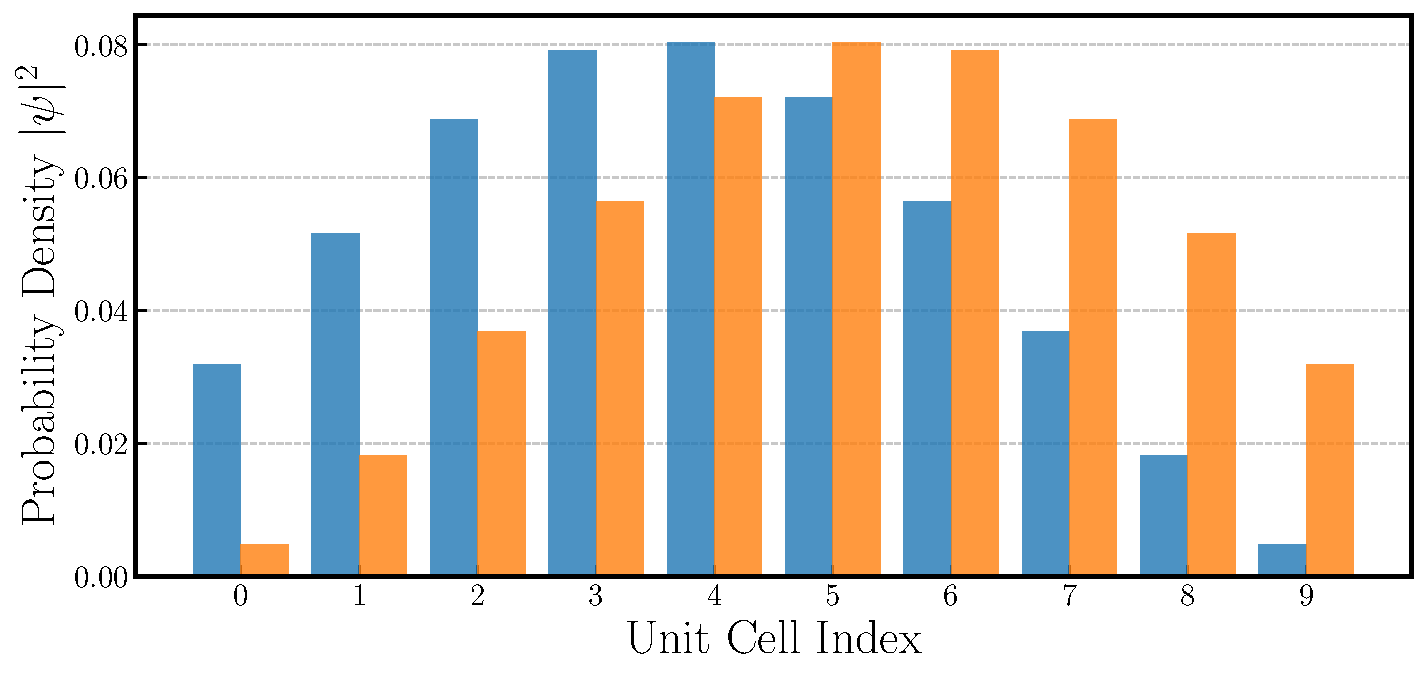
\includegraphics[width=\textwidth, max height=0.4\textheight, keepaspectratio]{Figures/probability_v=1.5_w=1.0_N=10.pdf}
        \caption{$v=1.5, w=1.0$}
    \end{subfigure}
    \caption{Probability distribution of the eigenstate corresponding to the lowest positive-energy eigenvalue for a finite SSH chain containing \(N=10\) unit cells. Edge localization is observed in the topological phase (\(v<w\)).}
    \label{fig:prob10}
\end{figure}

\begin{figure}[!htbp]
    \centering
    \begin{subfigure}[b]{0.48\textwidth}
        \centering
        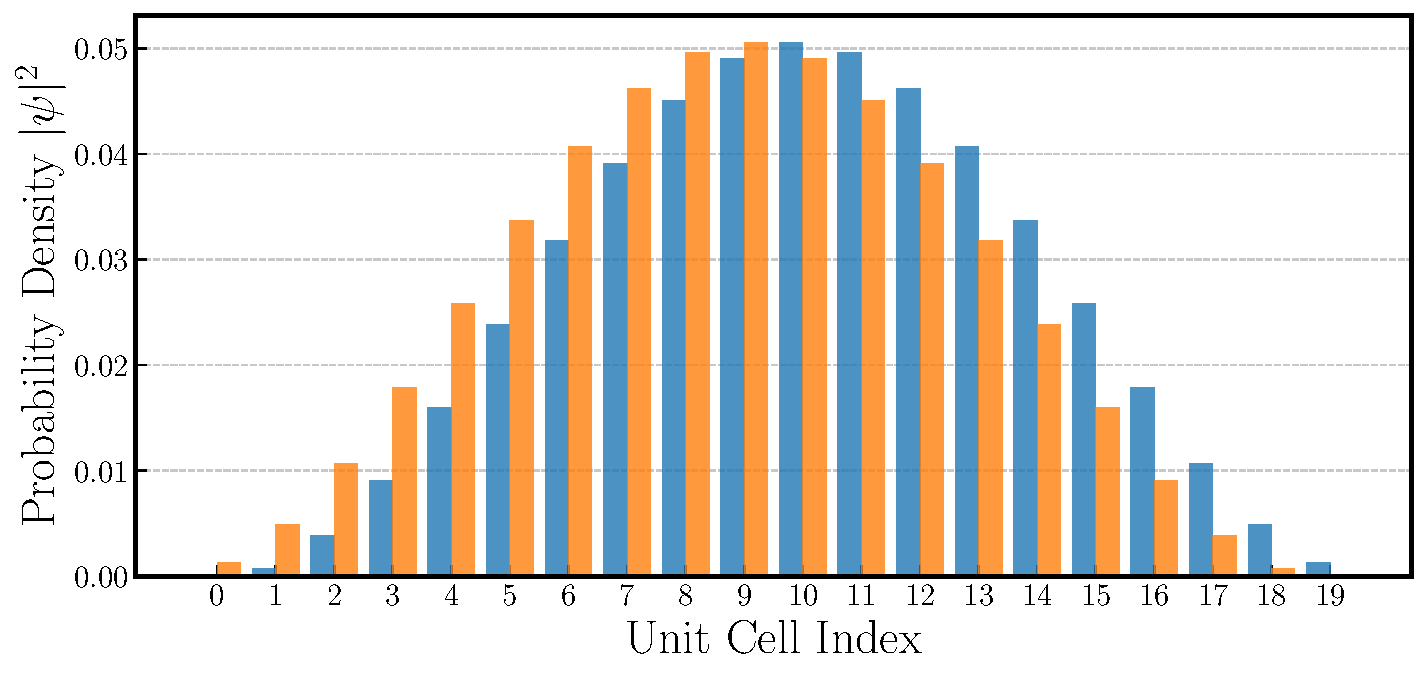
\includegraphics[width=\textwidth, max height=0.4\textheight, keepaspectratio]{Figures/probability_v=0.2_w=1.0_N=20.pdf}
        \caption{$v=0.2, w=1.0$}
    \end{subfigure}
    \hfill
    \begin{subfigure}[b]{0.48\textwidth}
        \centering
        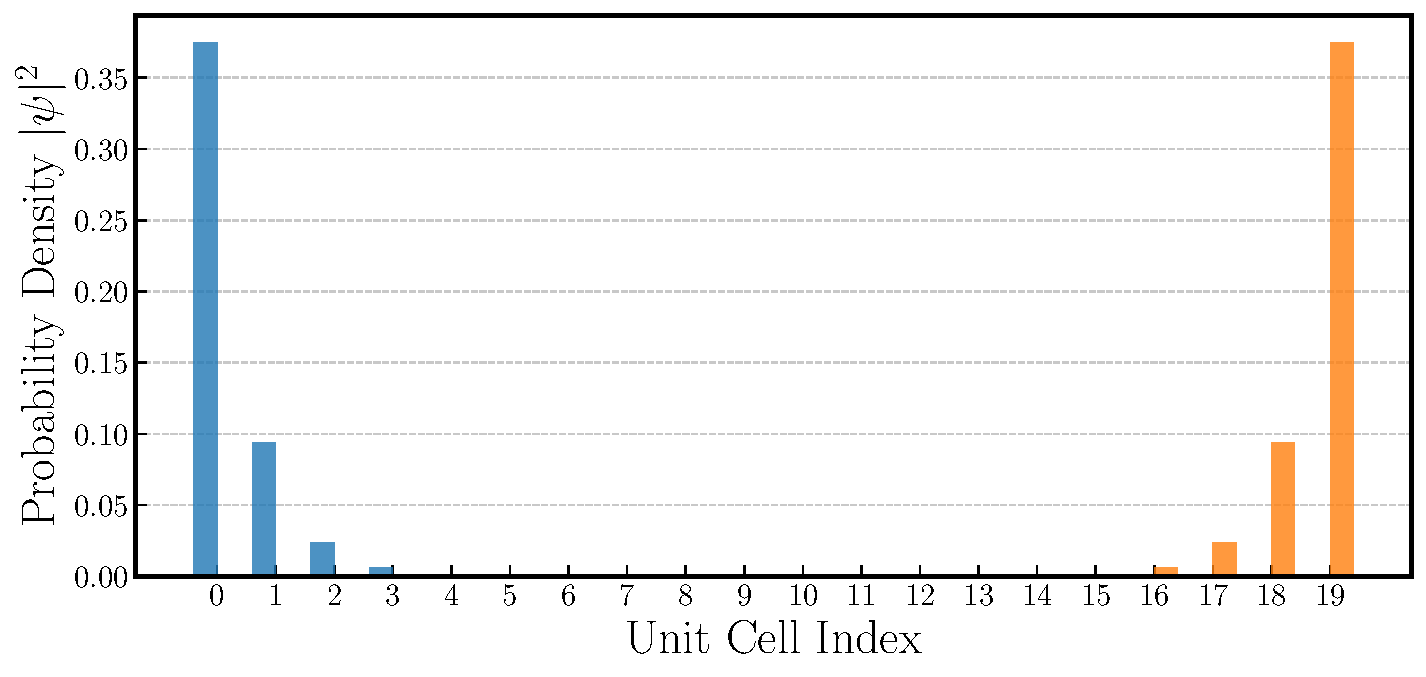
\includegraphics[width=\textwidth, max height=0.4\textheight, keepaspectratio]{Figures/probability_v=0.5_w=1.0_N=20.pdf}
        \caption{$v=0.5, w=1.0$}
    \end{subfigure}
    
    \vspace{0.4cm}
    
    \begin{subfigure}[b]{0.48\textwidth}
        \centering
        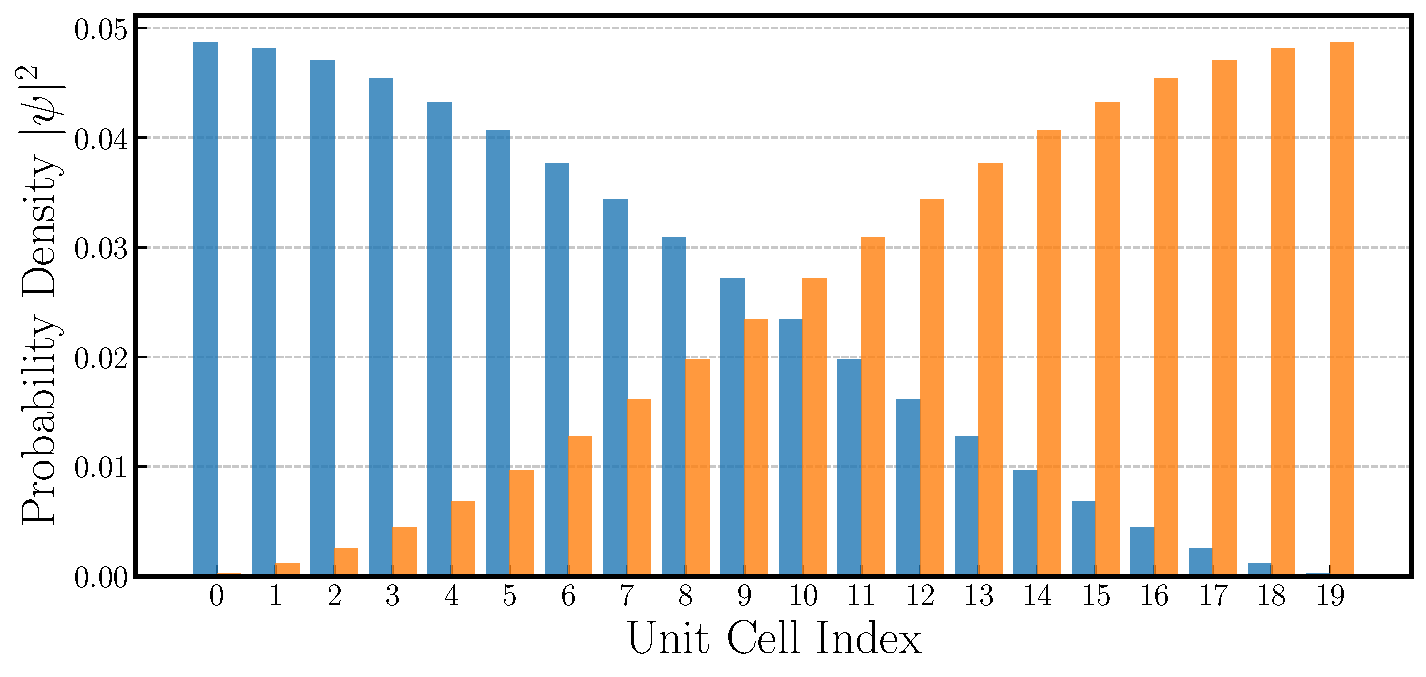
\includegraphics[width=\textwidth, max height=0.4\textheight, keepaspectratio]{Figures/probability_v=1.0_w=1.0_N=20.pdf}
        \caption{$v=1.0, w=1.0$}
    \end{subfigure}
    \hfill
    \begin{subfigure}[b]{0.48\textwidth}
        \centering
        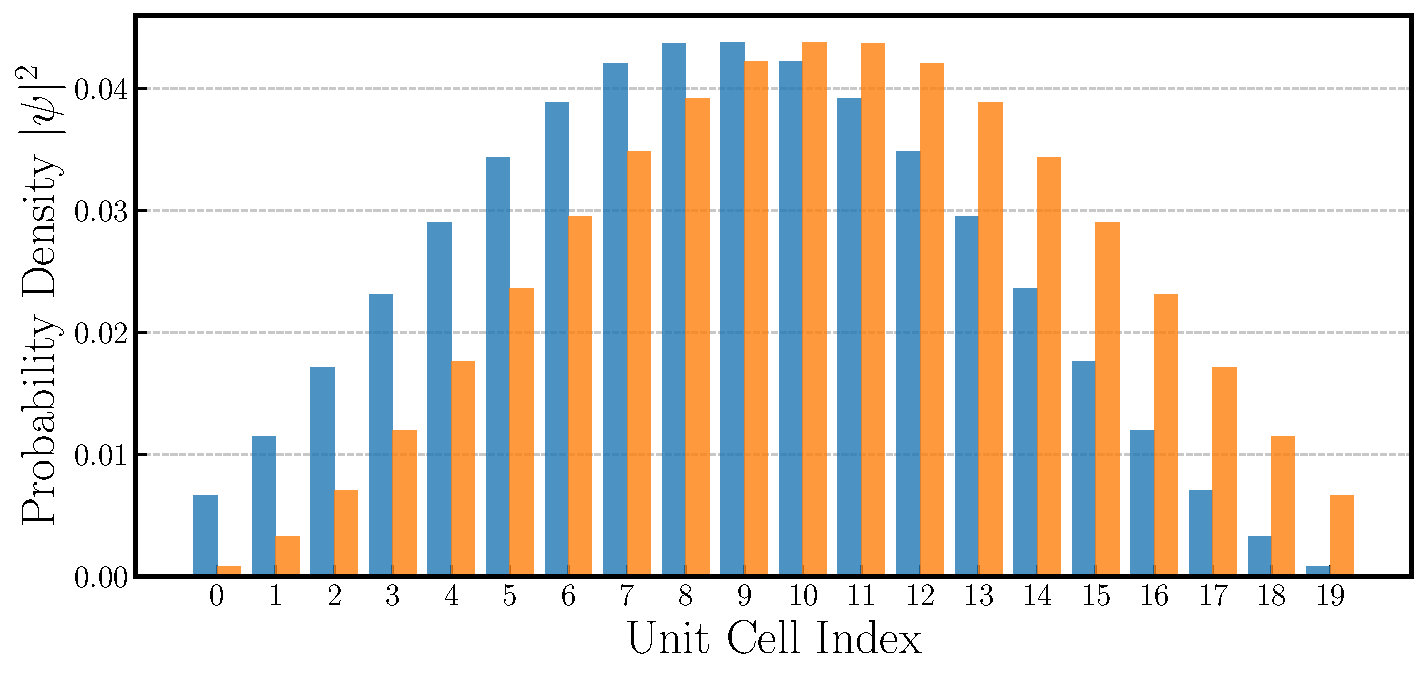
\includegraphics[width=\textwidth, max height=0.4\textheight, keepaspectratio]{Figures/probability_v=1.5_w=1.0_N=20.pdf}
        \caption{$v=1.5, w=1.0$}
    \end{subfigure}
    \caption{Probability distribution of the eigenstate corresponding to the lowest positive-energy eigenvalue for \(N=20\). The increased chain length leads to more strongly localized edge states and reduced overlap between opposite boundaries.}
    \label{fig:prob20}
\end{figure}
\FloatBarrier

\subsubsection{Preservation of Chiral Symmetry}

The finite SSH Hamiltonian retains the bipartite structure of the infinite lattice, containing hopping only between the two sublattices. Consequently, the chiral operator
\(\Gamma=\sigma_z\) continues to satisfy

\[
\Gamma H \Gamma^\dagger=-H,
\]

or equivalently,

\[
\{\Gamma,H\}=0.
\]
\
Therefore, the finite Hamiltonian preserves chiral symmetry. As a consequence, the energy spectrum remains symmetric about zero energy, with every positive-energy eigenstate having a corresponding negative-energy partner. The zero-energy edge states that appear in the topological phase are protected by this symmetry and remain pinned close to zero energy as long as the bulk energy gap remains open and the bipartite structure of the lattice is preserved.

\section{Extension of the SSH Model: Inclusion of an On-Site Potential}
\sectionmark{SSH Model with On-Site Potential}
\label{sec:onsite_potential}

In the previous sections, the SSH model was studied under the ideal
assumption that both sublattices possess zero on-site energies, so that
the Hamiltonian contains only nearest-neighbour hopping terms. We now extend
the model by introducing a staggered on-site potential, assigning an energy
$+u$ to every $A$ sublattice site and $-u$ to every $B$ sublattice site.
This simple extension allows us to investigate how an energy imbalance
between the two sublattices modifies the electronic and topological
properties of the SSH model.

\subsection{Real-space Hamiltonian}

Including  the on-site potential, the real-space Hamiltonian becomes

\begin{align}
\hat H
={}&
v\sum_{m=1}^{N}
\left(
|m,A\rangle\langle m,B|
+
|m,B\rangle\langle m,A|
\right)
+
w\sum_{m=1}^{N-1}
\left(
|m+1,A\rangle\langle m,B|
+
|m,B\rangle\langle m+1,A|
\right)
\nonumber\\[0.5em]
&+
u\sum_{m=1}^{N}
\left(
|m,A\rangle\langle m,A|
-
|m,B\rangle\langle m,B|
\right).
\end{align}

The first term describes the intracell hopping with amplitude $v$, while the second term describes the intercell hopping with amplitude $w$. The additional term introduces different on-site energies for the two sublattices, assigning an energy $+u$ to the $A$ sublattice and $-u$ to the $B$ sublattice. Unlike the hopping terms, this contribution acts locally on each lattice site and does not couple the two sublattices.

Physically, the staggered on-site potential represents an energy
imbalance between the two sublattices of the crystal. Instead of the
two lattice sites within each unit cell being energetically equivalent,
the A sublattice is assigned an energy $+u$, while the B sublattice is
assigned an energy $-u$. Such a staggered potential may arise in
materials where the two atoms occupying the unit cell are chemically
different, through interactions with an underlying substrate, or by the
application of an external electric field that breaks the equivalence
between the two sublattices.

Unlike the hopping terms, which couple neighbouring lattice sites, the
on-site potential acts locally on each lattice site and modifies only
its energy. Nevertheless, this additional term has profound
consequences, as it breaks the chiral symmetry responsible for the
topological protection of the SSH model.



\subsection{Momentum-Space Hamiltonian}

Since the bulk Hamiltonian possesses translational symmetry, Bloch's theorem
can again be applied \cite{asboth2015,ashcroft1976}. The external degree of
freedom is transformed from the real-space basis to the momentum-space basis
through the discrete Fourier transform,

\begin{equation}
\ket{k}
=
\frac{1}{\sqrt{N}}
\sum_{m=1}^{N}
e^{ikm}\ket{m},
\qquad
k=\frac{2\pi n}{N},
\quad
n=0,1,\dots,N-1.
\end{equation}

The Bloch eigenstates are therefore written as

\begin{equation}
\ket{\Psi_n(k)}
=
\ket{k}\otimes\ket{u_n(k)},
\qquad
\ket{u_n(k)}
=
a_n(k)\ket{A}
+
b_n(k)\ket{B}.
\end{equation}

Projecting the bulk Hamiltonian onto the Bloch basis gives

\begin{equation*}
H(k)
=
\bra{k}\hat{H}_{\mathrm{bulk}}\ket{k}.
\end{equation*}

The hopping terms are identical to those obtained for the SSH model,

\begin{align*}
\bra{k}
\left(
\sum_{m=1}^{N}\ket{m}\bra{m}
\right)
\ket{k}
&=1,\\[2mm]
\bra{k}
\left(
\sum_{m=1}^{N}\ket{m+1}\bra{m}
\right)
\ket{k}
&=e^{-ik},\\[2mm]
\bra{k}
\left(
\sum_{m=1}^{N}\ket{m}\bra{m+1}
\right)
\ket{k}
&=e^{ik}.
\end{align*}

The additional staggered on-site potential contributes

\begin{equation*}
u
\sum_{m=1}^{N}
\ket{m}\bra{m}
\otimes
\left(
\ket{A}\bra{A}
-
\ket{B}\bra{B}
\right).
\end{equation*}

Since

\begin{equation*}
\bra{k}
\left(
\sum_{m=1}^{N}\ket{m}\bra{m}
\right)
\ket{k}
=1,
\end{equation*}

the on-site potential remains unchanged after the Fourier transformation,

\begin{equation*}
u
\left(
\ket{A}\bra{A}
-
\ket{B}\bra{B}
\right).
\end{equation*}

Substituting these results into the Hamiltonian gives

\begin{align*}
H(k)
&=
u
\left(
\ket{A}\bra{A}
-
\ket{B}\bra{B}
\right)
\\
&\quad
+
v
\left(
\ket{B}\bra{A}
+
\ket{A}\bra{B}
\right)
\\
&\quad
+
w
\left(
e^{-ik}\ket{A}\bra{B}
+
e^{ik}\ket{B}\bra{A}
\right).
\end{align*}

Using

\[
\ket{A}\bra{A}
=
\begin{pmatrix}
1&0\\
0&0
\end{pmatrix},
\qquad
\ket{B}\bra{B}
=
\begin{pmatrix}
0&0\\
0&1
\end{pmatrix},
\]

together with

\[
\ket{A}\bra{B}
=
\begin{pmatrix}
0&1\\
0&0
\end{pmatrix},
\qquad
\ket{B}\bra{A}
=
\begin{pmatrix}
0&0\\
1&0
\end{pmatrix},
\]

the momentum-space Hamiltonian becomes

\begin{equation}
H(k)
=
\begin{pmatrix}
u &
v+we^{-ik}
\\
v+we^{ik} &
-u
\end{pmatrix},
\label{eq:momentum_space_Hamiltonian_u}
\end{equation}
Compared to the SSH Hamiltonian, the only modification is the appearance of the diagonal on-site potential $\pm u$, while the hopping terms remain unchanged.

The Schr\"odinger equation in momentum space is therefore

\begin{equation*}
H(k)\ket{u_n(k)}
=
E_n(k)\ket{u_n(k)},
\end{equation*}

which determines the bulk energy spectrum and the corresponding eigenstates of the SSH model with a staggered on-site potential.



\subsection{Representation in Terms of Pauli Matrices}

The momentum-space Hamiltonian may be expressed in terms of the Pauli matrices as

\[
H(k)
=
d_x(k)\sigma_x
+
d_y(k)\sigma_y
+
u\sigma_z,
\]

where

\[
d_x(k)=v+w\cos k,
\]

and

\[
d_y(k)=w\sin k.
\]

The additional term proportional to $\sigma_z$ originates from the staggered
on-site potential and represents the energy difference between the two
sublattices.

\subsection{Effect on Chiral Symmetry}

For the original SSH Hamiltonian, the chiral symmetry condition

\[
\{\Gamma,H(k)\}=0,
\]

is satisfied, where

\[
\Gamma=\sigma_z.
\]

For the modified Hamiltonian,

\[
H(k)
=
d_x(k)\sigma_x
+
d_y(k)\sigma_y
+
u\sigma_z,
\]

the anticommutator is

\begin{align}
\{\Gamma,H(k)\}
&=
\sigma_zH(k)+H(k)\sigma_z
\\
&=
\sigma_z
\left(
d_x\sigma_x+d_y\sigma_y+u\sigma_z
\right)
+
\left(
d_x\sigma_x+d_y\sigma_y+u\sigma_z
\right)
\sigma_z
\\
&=
d_x(\sigma_z\sigma_x+\sigma_x\sigma_z)
+
d_y(\sigma_z\sigma_y+\sigma_y\sigma_z)
+
u(\sigma_z^2+\sigma_z^2).
\end{align}

Using the identities

\[
\{\sigma_z,\sigma_x\}=0,\qquad
\{\sigma_z,\sigma_y\}=0,\qquad
\sigma_z^2=I,
\]

we obtain

\[
\{\Gamma,H(k)\}=2uI.
\]

Hence, for

\[
u\neq0,
\]

the operator $\Gamma=\sigma_z$ no longer anticommutes with the Hamiltonian.

One may ask whether there exists another operator that satisfies the chiral
symmetry condition. Consider the most general Hermitian unitary operator

\[
\Gamma
=
n_x\sigma_x+n_y\sigma_y+n_z\sigma_z,
\]

where

\[
n_x^2+n_y^2+n_z^2=1.
\]

Using the Pauli matrix anticommutation relations,

\[
\{\sigma_i,\sigma_j\}=2\delta_{ij}I,
\]

the anticommutator becomes

\[
\{\Gamma,H(k)\}
=
2\left(
n_xd_x(k)+n_yd_y(k)+n_zu
\right)I.
\]

For chiral symmetry to exist, this expression must vanish for every value of
$k$, giving

\[
n_xd_x(k)+n_yd_y(k)+n_zu=0.
\]

Substituting

\[
d_x(k)=v+w\cos k,
\qquad
d_y(k)=w\sin k,
\]

yields

\[
n_x(v+w\cos k)
+
n_yw\sin k
+
n_zu
=0.
\]

Since the functions \(1\), \(\cos k\), and \(\sin k\) are linearly
independent, their coefficients must vanish separately. Thus,

\[
n_x=0,\qquad
n_y=0,\qquad
n_zu=0.
\]

For

\[
u\neq0,
\]

it follows that

\[
n_z=0,
\]

which contradicts the normalization condition

\[
n_x^2+n_y^2+n_z^2=1.
\]

Therefore, no nontrivial Hermitian unitary operator exists that anticommutes
with the Hamiltonian. The staggered on-site potential completely breaks the
chiral symmetry, and consequently the Hamiltonian can no longer be written in
a purely off-diagonal form.


\subsection{Loss of the Winding Number}

For the original SSH model, the momentum-space Hamiltonian may be written as

\[
H(k)=d_x(k)\sigma_x+d_y(k)\sigma_y,
\]

so that the vector

\[
\mathbf d(k)=\left(d_x(k),d_y(k),0\right)
\]

is confined entirely to the $d_x$--$d_y$ plane. As the crystal momentum
varies across the Brillouin zone, the normalized vector
$\hat{\mathbf d}(k)$ traces a closed curve in this plane, and the
winding number counts how many times this curve encircles the origin.

After introducing the staggered on-site potential, the Hamiltonian
becomes

\[
H(k)=d_x(k)\sigma_x+d_y(k)\sigma_y+u\sigma_z,
\]

and the corresponding vector becomes

\[
\mathbf d(k)=\left(d_x(k),d_y(k),u\right).
\]

The trajectory is therefore no longer confined to a two-dimensional
plane but instead forms a closed curve in three-dimensional space. Since
the original winding number is defined only for planar trajectories, it
is no longer applicable once the $\sigma_z$ term is present.

Thus, the staggered on-site potential breaks chiral symmetry and
removes the topological invariant that distinguishes the two phases of
the SSH model.


\subsection{Energy Eigenvalues}

The energy eigenvalues are obtained by solving the eigenvalue equation

\[
H(k)|\psi(k)\rangle
=
E(k)|\psi(k)\rangle,
\]

or equivalently,

\[
\det\!\left[H(k)-EI\right]=0.
\]

Using the momentum-space Hamiltonian

\[
H(k)
=
\begin{pmatrix}
u &
v+we^{-ik}\\
v+we^{ik} &
-u
\end{pmatrix},
\]

we obtain

\[
\det
\begin{pmatrix}
u-E &
v+we^{-ik}\\
v+we^{ik} &
-u-E
\end{pmatrix}
=0.
\]

Evaluating the determinant,

\[
(u-E)(-u-E)
-
(v+we^{-ik})(v+we^{ik})
=0.
\]

Since

\[
(v+we^{-ik})(v+we^{ik})
=
v^2+w^2+2vw\cos k,
\]

the characteristic equation becomes

\[
E^2
=
u^2
+
v^2
+
w^2
+
2vw\cos k.
\]

Hence, the energy eigenvalues are

\[
    E_{\pm}(k)
    =
    \pm
    \sqrt{
    u^2
    +
    v^2
    +
    w^2
    +
    2vw\cos k
    }.
\]

Compared to the original SSH model, the staggered on-site potential
introduces an additional contribution of $u^2$ under the square root.
The modified expression reduces to the standard SSH dispersion relation in
the limit $u=0$.

\subsection{Energy Spectrum}

The energy spectrum of the finite SSH chain was computed numerically using
the analytical expression derived above,

\[
E_{\pm}(k)
=
\pm
\sqrt{
u^2
+
v^2
+
w^2
+
2vw\cos k
},
\]

for the parameter values

\[
v=0.2,\qquad
w=1,
\]

and for three different values of the staggered on-site potential,

\[
u=0,\qquad
u=0.1,\qquad
u=-0.1.
\]

The resulting energy spectra of the finite SSH chain are shown in
\cref{fig:energy_spectrum_onsite}.

\begin{figure}[htbp]
    \centering

    % First row
    \begin{subfigure}[b]{0.48\textwidth}
        \centering
        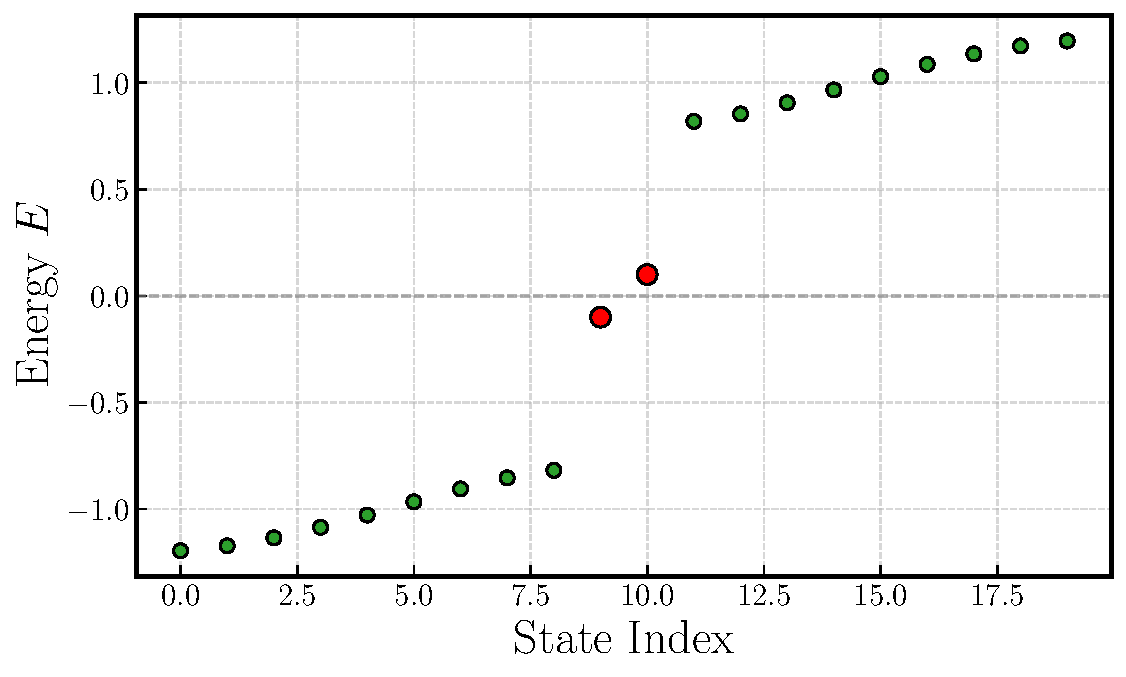
\includegraphics[width=\textwidth]{Figures/onsite_potential/spectrum_v=0.2_w=1.0_u=-0.1_N=10.pdf}
        \caption{$u=-0.1,\;N=10$}
        \label{fig:onsite_a}
    \end{subfigure}
    \hfill
    \begin{subfigure}[b]{0.48\textwidth}
        \centering
        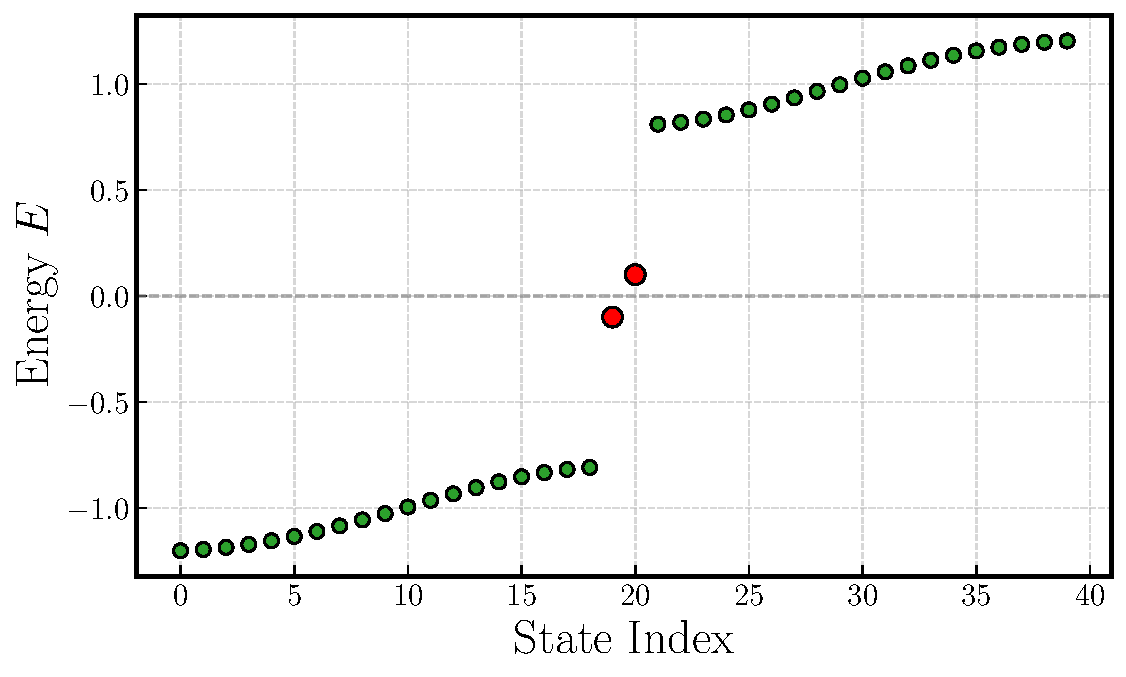
\includegraphics[width=\textwidth]{Figures/onsite_potential/spectrum_v=0.2_w=1.0_u=-0.1_N=20.pdf}
        \caption{$u=-0.1,\;N=20$}
        \label{fig:onsite_b}
    \end{subfigure}

    \vspace{0.4cm}

    % Second row
    \begin{subfigure}[b]{0.48\textwidth}
        \centering
        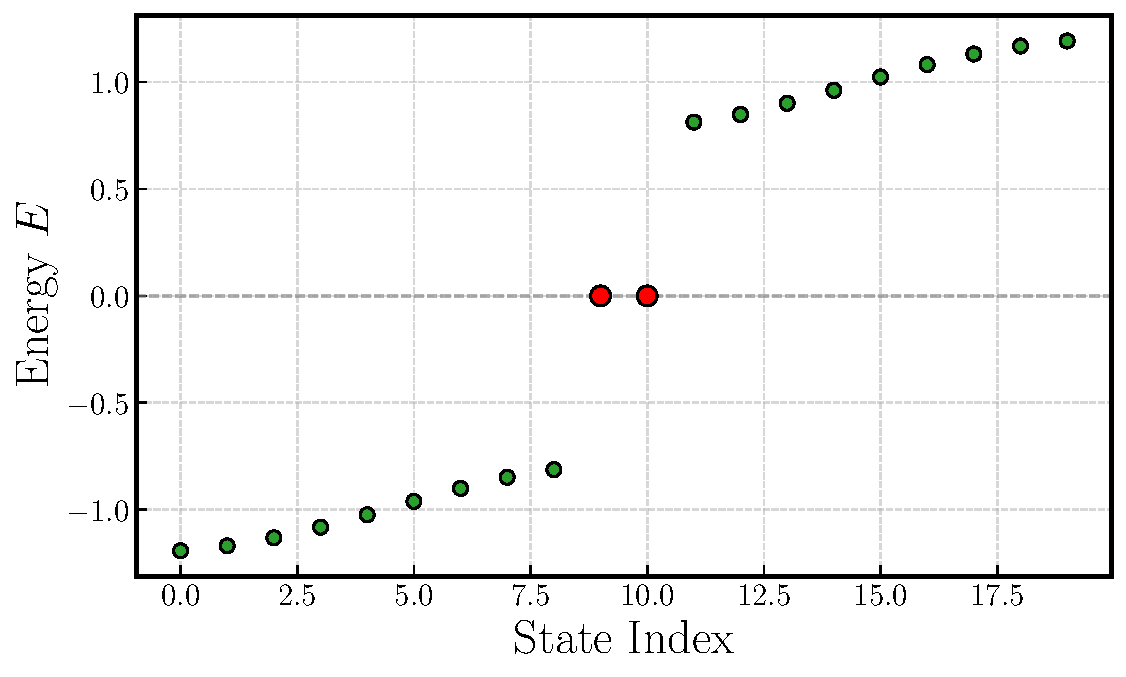
\includegraphics[width=\textwidth]{Figures/onsite_potential/spectrum_v=0.2_w=1.0_u=0.0_N=10.pdf}
        \caption{$u=0,\;N=10$}
        \label{fig:onsite_c}
    \end{subfigure}
    \hfill
    \begin{subfigure}[b]{0.48\textwidth}
        \centering
        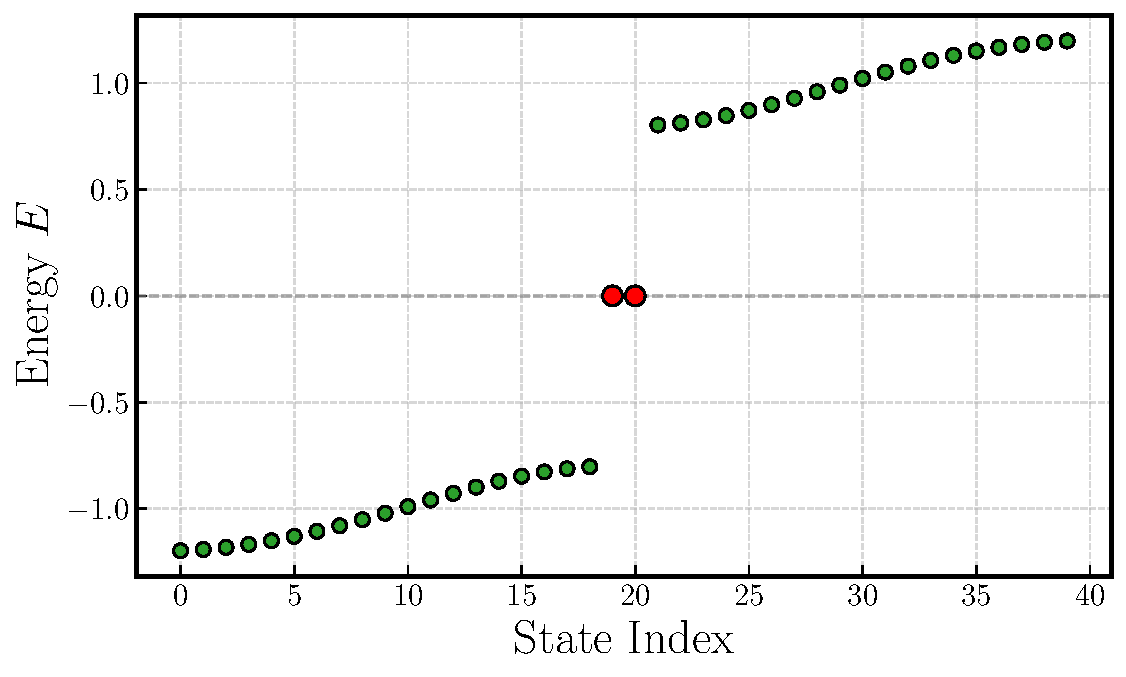
\includegraphics[width=\textwidth]{Figures/onsite_potential/spectrum_v=0.2_w=1.0_u=0.0_N=20.pdf}
        \caption{$u=0,\;N=20$}
        \label{fig:onsite_d}
    \end{subfigure}

    \vspace{0.4cm}

    % Third row
    \begin{subfigure}[b]{0.48\textwidth}
        \centering
        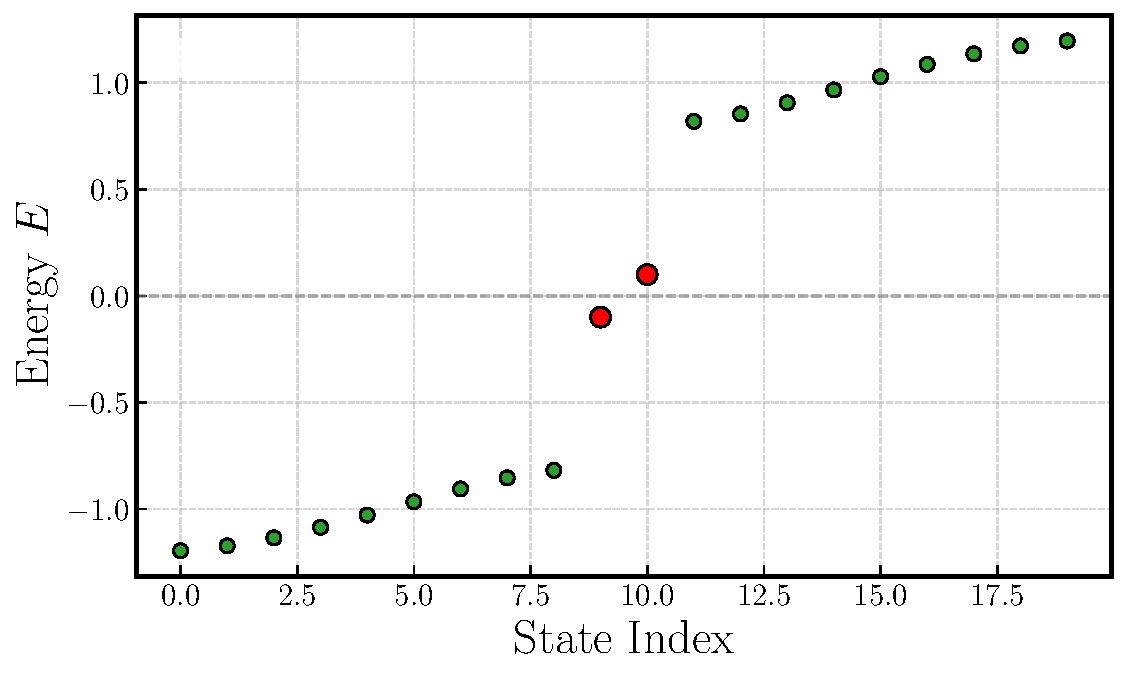
\includegraphics[width=\textwidth]{Figures/onsite_potential/spectrum_v=0.2_w=1.0_u=0.1_N=10.pdf}
        \caption{$u=0.1,\;N=10$}
        \label{fig:onsite_e}
    \end{subfigure}
    \hfill
    \begin{subfigure}[b]{0.48\textwidth}
        \centering
        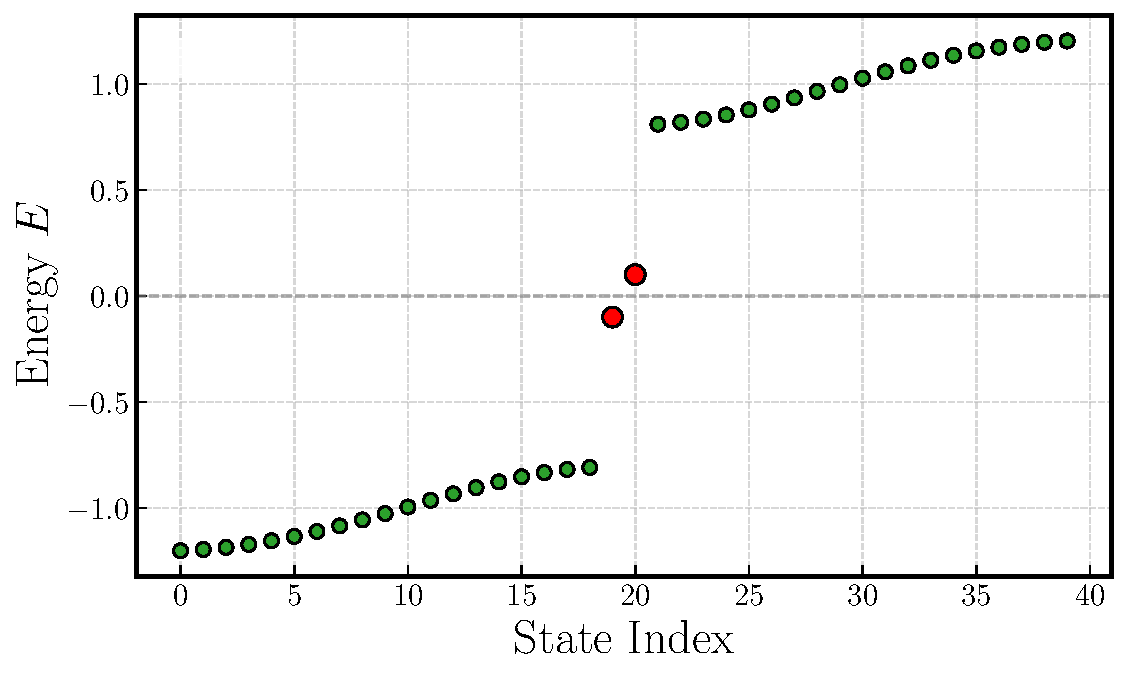
\includegraphics[width=\textwidth]{Figures/onsite_potential/spectrum_v=0.2_w=1.0_u=0.1_N=20.pdf}
        \caption{$u=0.1,\;N=20$}
        \label{fig:onsite_f}
    \end{subfigure}

    \caption{Energy spectra of the finite SSH chain with a staggered on-site potential
for $v=0.2$ and $w=1.0$. The left column corresponds to a chain of
$N=10$ unit cells, while the right column corresponds to $N=20$ unit
cells. The rows show the spectra for $u=-0.1$, $u=0$, and $u=0.1$,
respectively. The red points indicate the edge states.}
    \label{fig:energy_spectrum_onsite}
\end{figure}

For $u=0$, the spectrum reduces to that of the standard SSH model discussed
previously, with the edge states remaining at zero energy. Introducing a
finite staggered on-site potential shifts these edge states away from zero
energy, while the bulk spectrum remains qualitatively similar. Since the
energy eigenvalues depend on $u^2$, the spectra for $u=0.1$ and $u=-0.1$
are identical, with the sign of the on-site potential affecting the
eigenstates rather than the eigenvalues.

\subsection{Eigenstates}

To examine the effect of the staggered on-site potential on the edge
states of the SSH model, the finite-chain Hamiltonian was numerically
diagonalized for

\[
v=0.2,\qquad
w=1,
\]

using the same values of the on-site potential,

\[
u=-0.1,\qquad
u=0,\qquad
u=0.1.
\]

The probability density associated with a normalized eigenstate is given by

\[
P_n=|\psi_n|^2,
\]

where $\psi_n$ denotes the amplitude of the eigenvector at the $n$th lattice
site. The probability distributions of the positive- and negative-energy
edge states are shown in \cref{fig:onsite_eigenstates_N10,fig:onsite_eigenstates_N20}.

\begin{figure}[htbp]
    \centering

    \begin{subfigure}[b]{0.95\textwidth}
        \centering
        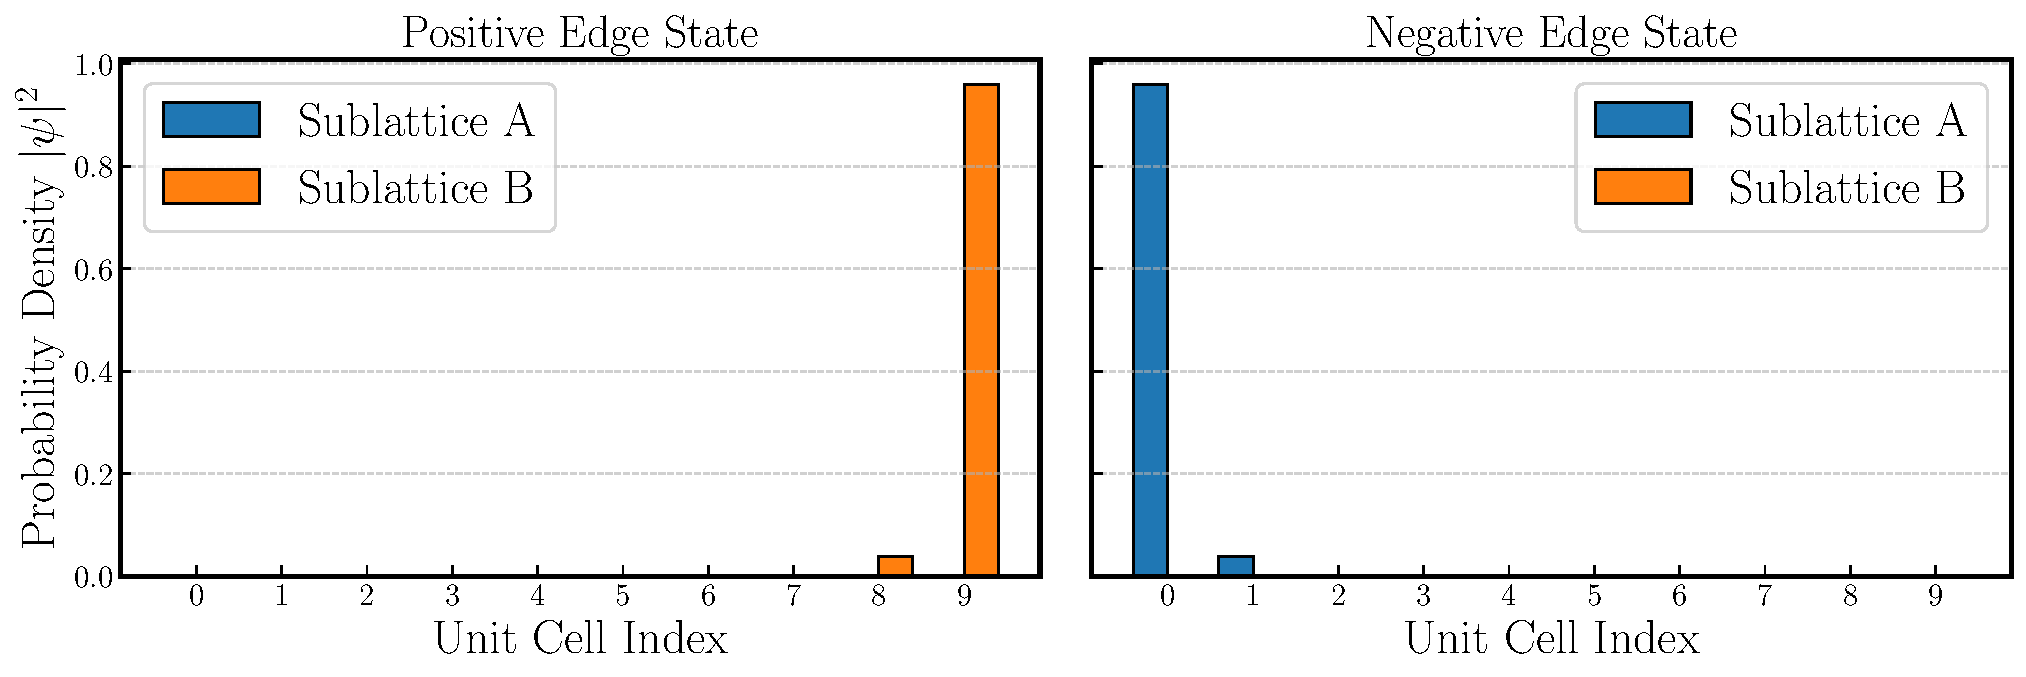
\includegraphics[width=\textwidth]{Figures/onsite_potential/edge_states_v=0.2_w=1.0_u=-0.1_N=10.pdf}
        \caption{$u=-0.1$}
        \label{fig:edge10_a}
    \end{subfigure}

    \vspace{0.15cm}

    \begin{subfigure}[b]{0.95\textwidth}
        \centering
        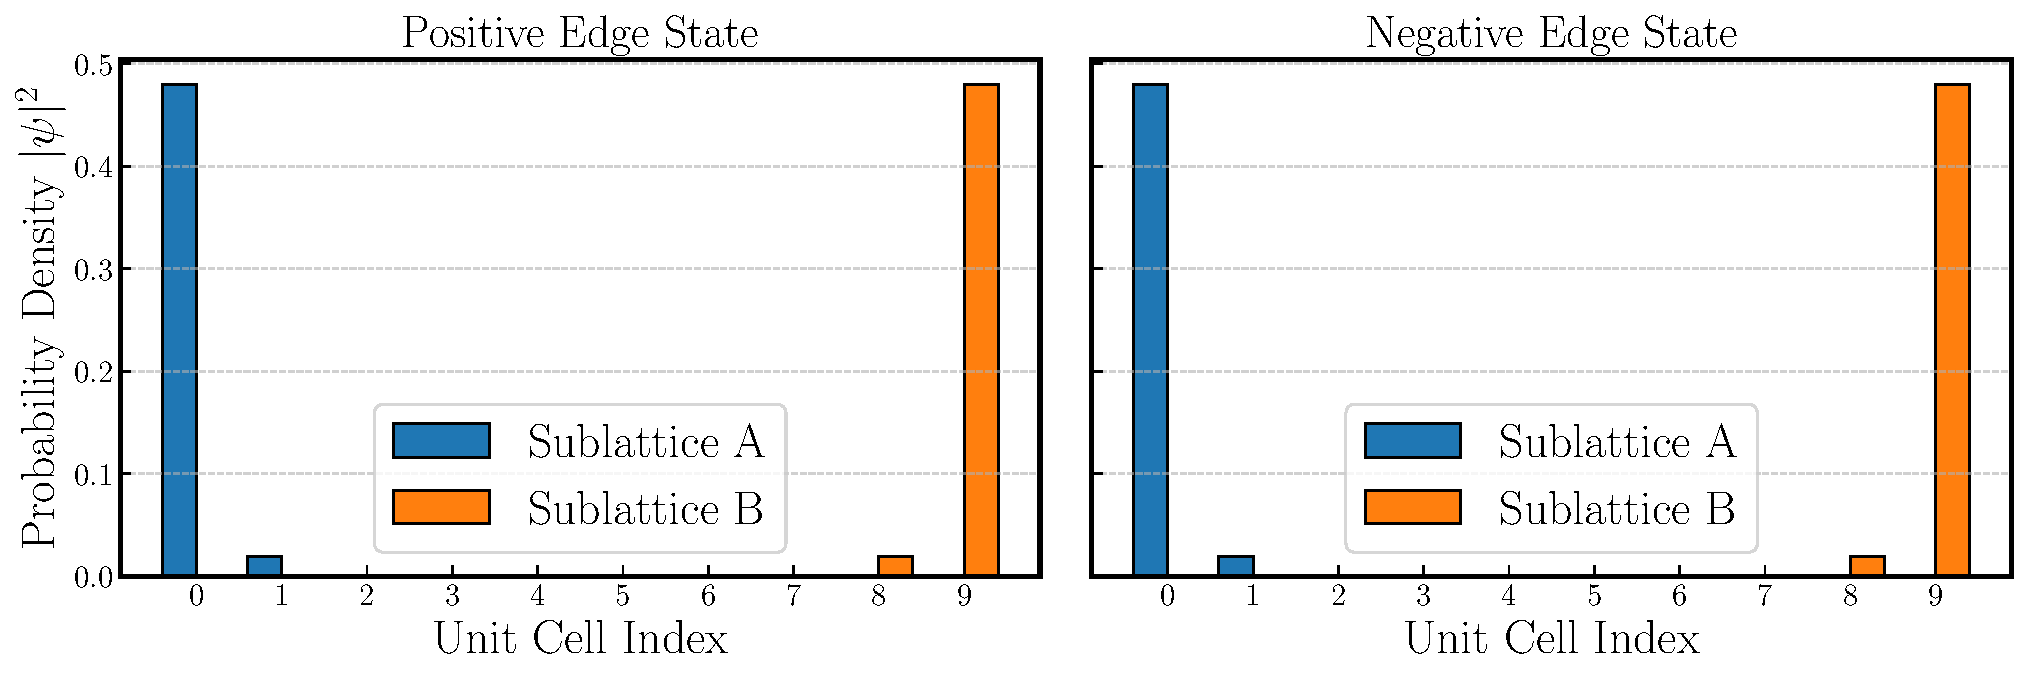
\includegraphics[width=\textwidth]{Figures/onsite_potential/edge_states_v=0.2_w=1.0_u=0.0_N=10.pdf}
        \caption{$u=0$}
        \label{fig:edge10_b}
    \end{subfigure}

    \vspace{0.15cm}

    \begin{subfigure}[b]{0.95\textwidth}
        \centering
        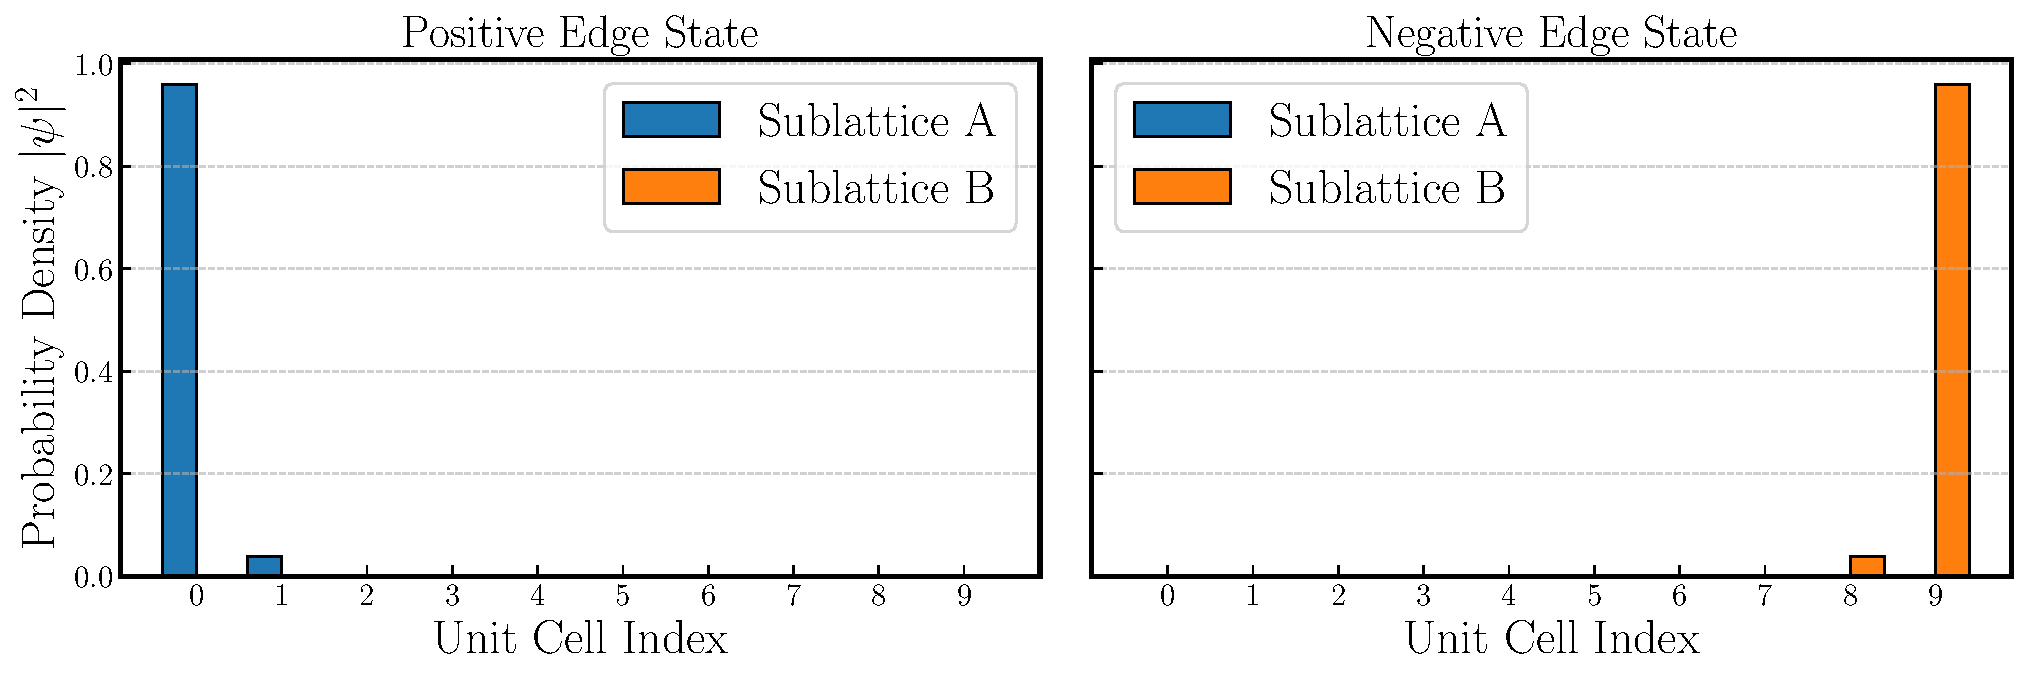
\includegraphics[width=\textwidth]{Figures/onsite_potential/edge_states_v=0.2_w=1.0_u=0.1_N=10.pdf}
        \caption{$u=0.1$}
        \label{fig:edge10_c}
    \end{subfigure}

    \caption{Probability density of the positive- and negative-energy edge states of the finite SSH chain containing $N=10$ unit cells for $v=0.2$ and $w=1.0$. The three panels correspond to $u=-0.1$, $u=0$, and $u=0.1$, respectively.}
    \label{fig:onsite_eigenstates_N10}
\end{figure}
\begin{figure}[htbp]
    \centering

    \begin{subfigure}[b]{0.95\textwidth}
        \centering
        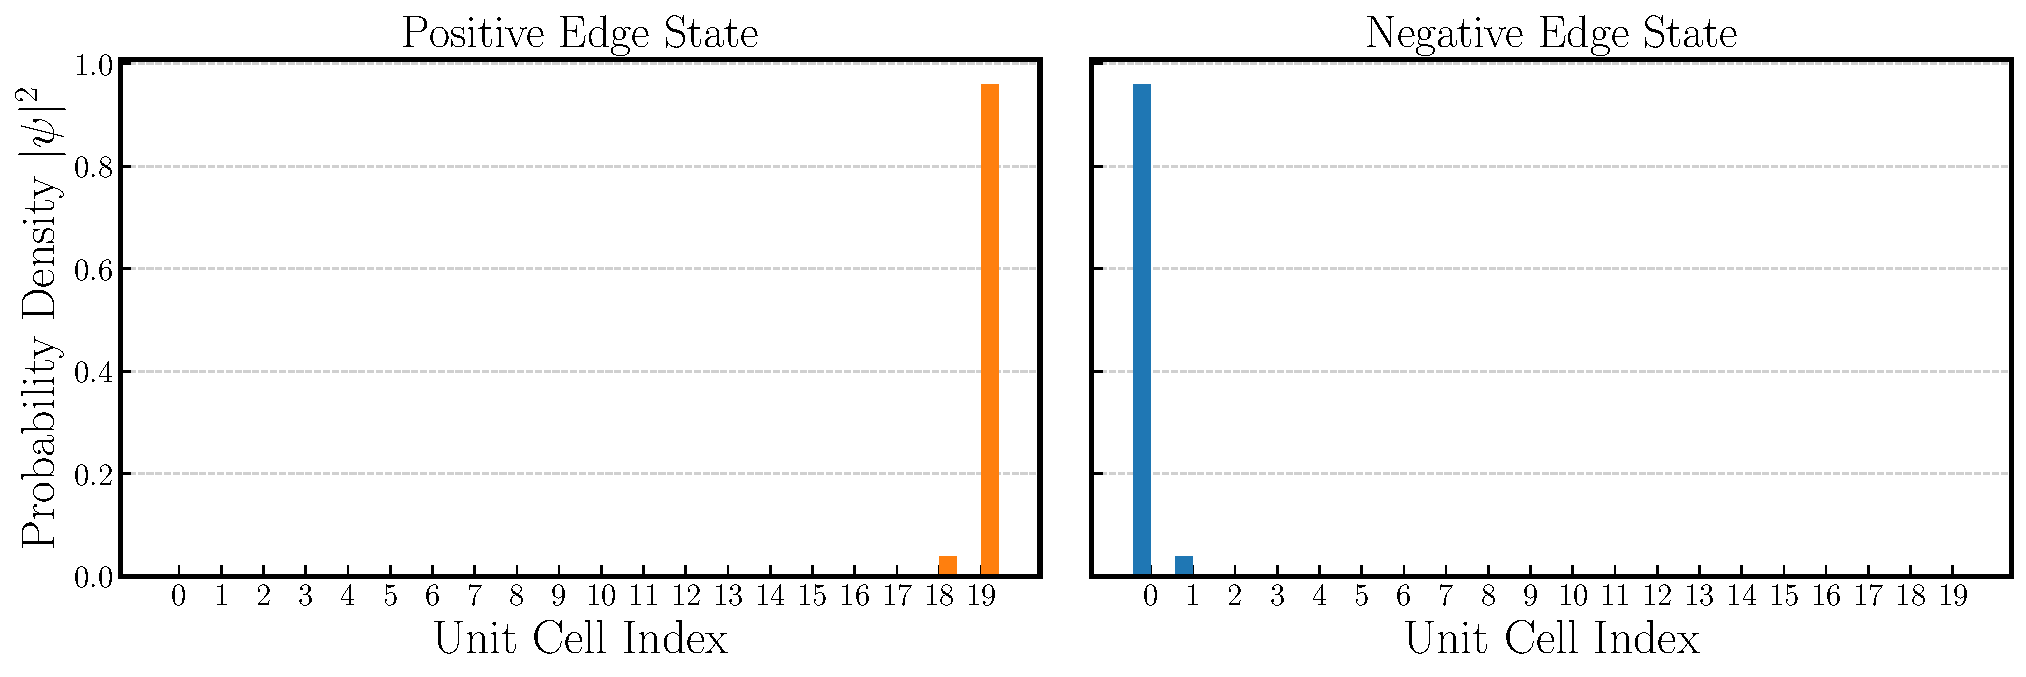
\includegraphics[width=\textwidth]{Figures/onsite_potential/edge_states_v=0.2_w=1.0_u=-0.1_N=20.pdf}
        \caption{$u=-0.1$}
        \label{fig:edge20_a}
    \end{subfigure}

    \vspace{0.15cm}

    \begin{subfigure}[b]{0.95\textwidth}
        \centering
        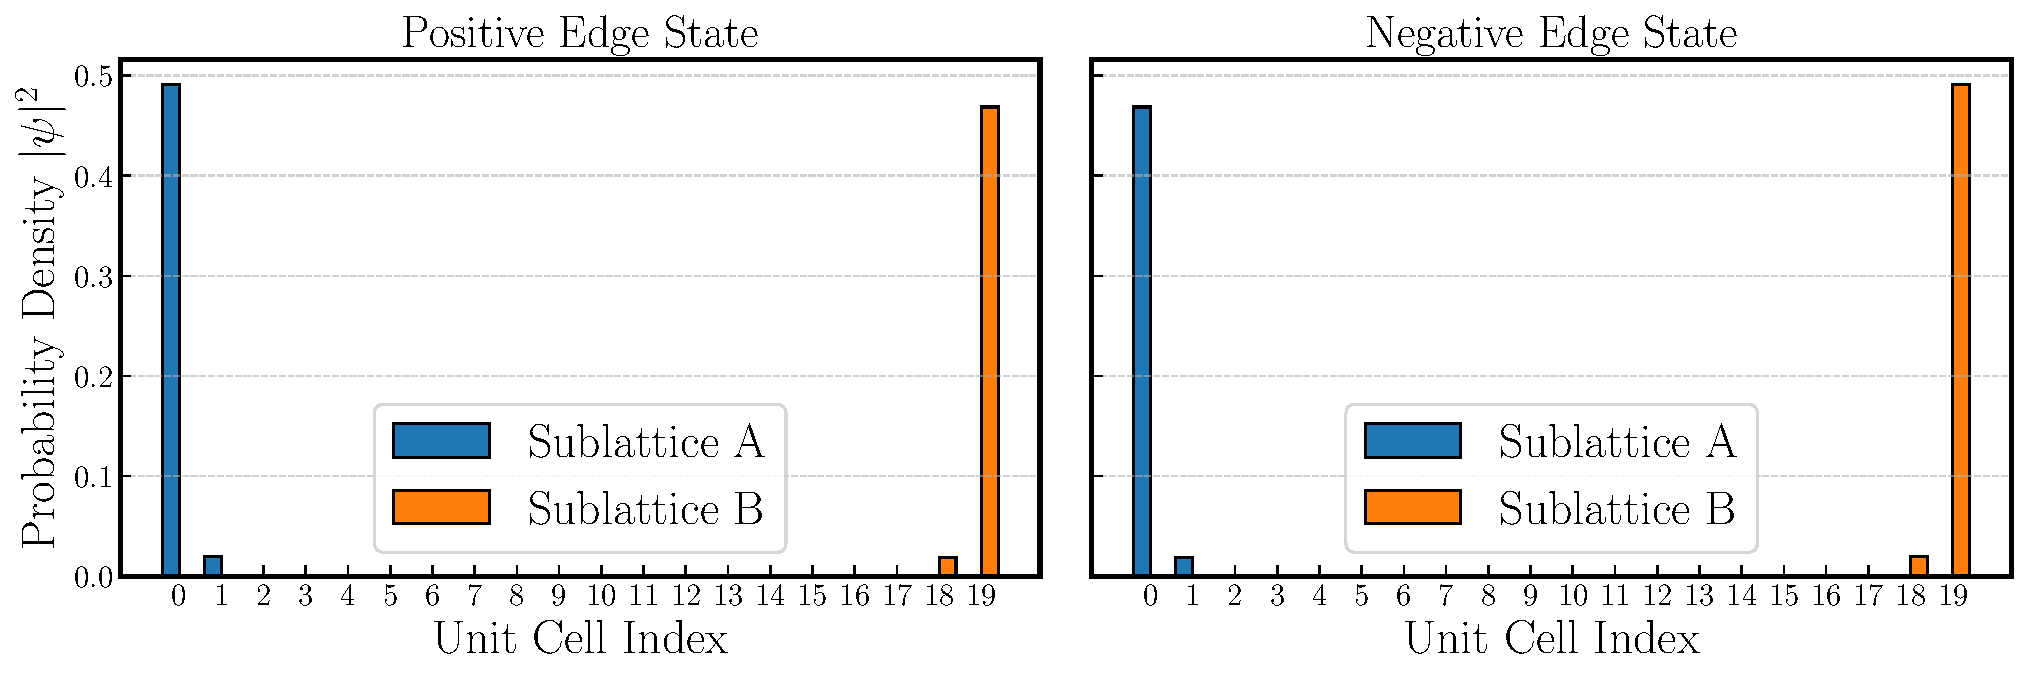
\includegraphics[width=\textwidth]{Figures/onsite_potential/edge_states_v=0.2_w=1.0_u=0.0_N=20.pdf}
        \caption{$u=0$}
        \label{fig:edge20_b}
    \end{subfigure}

    \vspace{0.15cm}

    \begin{subfigure}[b]{0.95\textwidth}
        \centering
        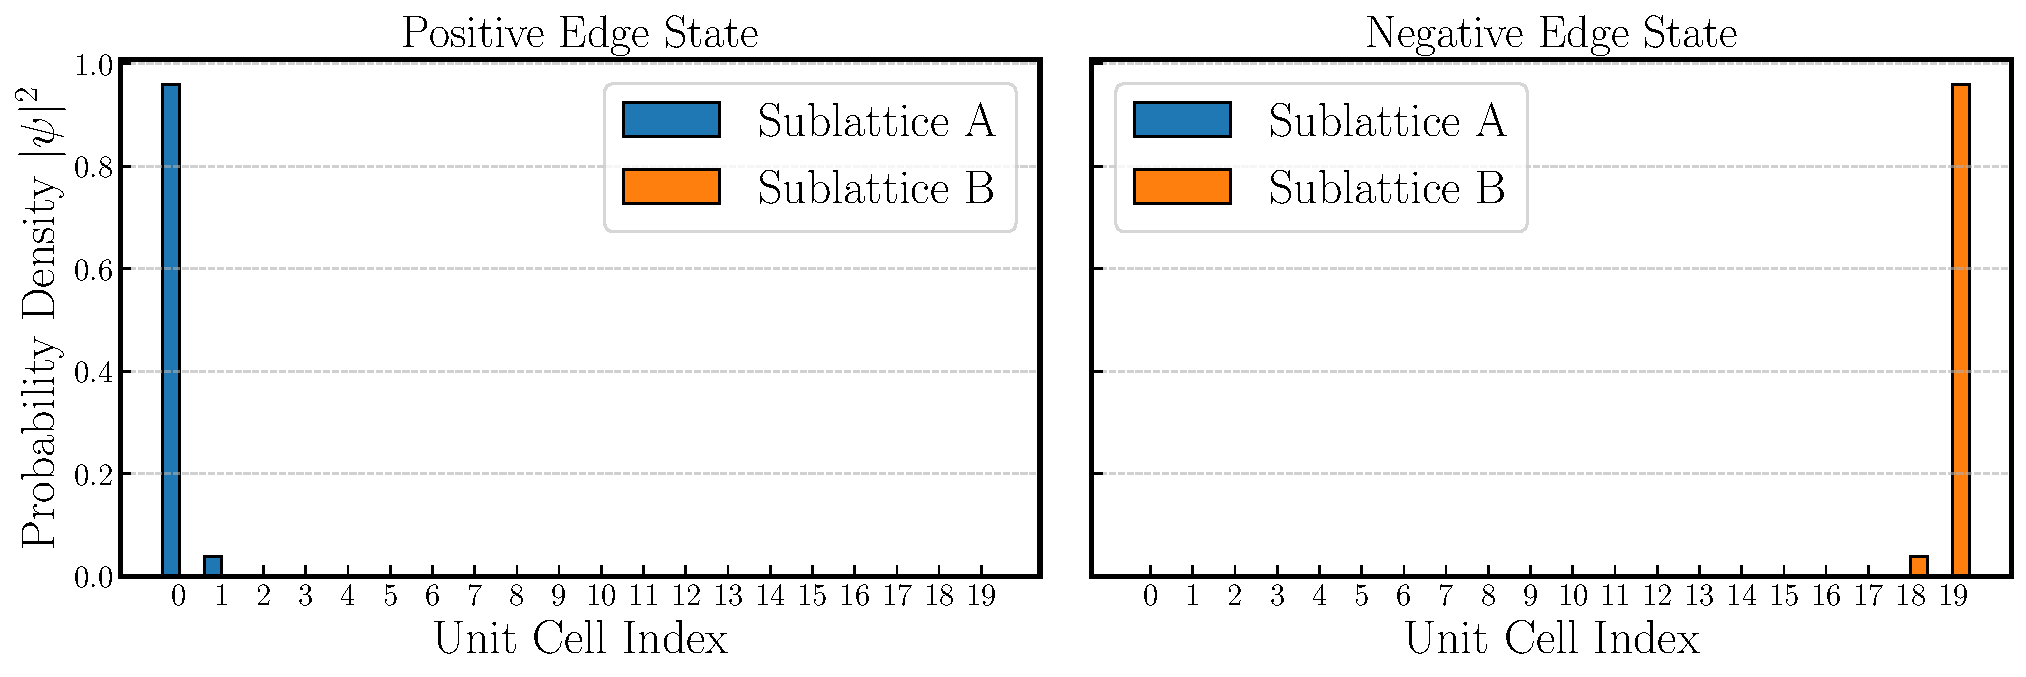
\includegraphics[width=\textwidth]{Figures/onsite_potential/edge_states_v=0.2_w=1.0_u=0.1_N=20.pdf}
        \caption{$u=0.1$}
        \label{fig:edge20_c}
    \end{subfigure}

    \caption{Probability density of the positive- and negative-energy edge states of the finite SSH chain containing $N=20$ unit cells for $v=0.2$ and $w=1.0$. The three panels correspond to $u=-0.1$, $u=0$, and $u=0.1$, respectively.}
    \label{fig:onsite_eigenstates_N20}
\end{figure}

As shown in \cref{fig:onsite_eigenstates_N10,fig:onsite_eigenstates_N20}, the edge states remain strongly localized at the ends of the chain for all three values of the staggered on-site potential. The probability density decays rapidly into the bulk, indicating that the edge localization is largely unaffected by the introduction of the on-site potential.

For $u=0$, corresponding to the original SSH model, the two edge states are localized at opposite ends of the chain and occupy opposite sublattices. When a finite staggered on-site potential is introduced, the edge states remain localized at the boundaries; however, the sublattice on which the positive- and negative-energy edge states are concentrated depends on the sign of u. Reversing the sign of the on-site potential exchanges the sublattice character of the two edge states while preserving their boundary localization.

Unlike the chiral-symmetric SSH model, the edge states are no longer pinned to zero energy. In the original SSH model, chiral symmetry ensures that every positive-energy eigenstate has a corresponding negative-energy partner, forcing the topological edge states to lie exactly at zero energy. The staggered on-site potential introduces a diagonal term proportional to $\sigma_z$, breaking chiral symmetry and removing the spectral symmetry about zero energy. Consequently, the edge-state energies shift away from zero while the states remain strongly localized near the boundaries for the parameter values considered.

These results show that the staggered on-site potential primarily modifies the energies and sublattice character of the edge states, while their spatial localization is largely preserved within the range of u studied.

\FloatBarrier


\subsection{Winding Number}

For the chiral-symmetric SSH model (\(u=0\)), the topological phase is
characterized by the winding number, which counts the number of times the
normalized vector

\[
\hat{\mathbf d}(k)=\frac{\mathbf d(k)}{|\mathbf d(k)|}
\]

winds around the origin as the crystal momentum traverses the first
Brillouin zone. The winding number is given by

\begin{equation}
\nu
=
\frac{1}{2\pi}
\int_{-\pi}^{\pi}
\left(
\hat{\mathbf d}
\times
\frac{d\hat{\mathbf d}}{dk}
\right)_{z}
dk.
\label{eq:winding_number}
\end{equation}

For the parameter values

\[
v=0.2,\qquad
w=1,
\]

the numerical evaluation of \cref{eq:winding_number} gives

\[
\nu=1,
\]

confirming that the system is in the topological phase.

When a staggered on-site potential is introduced, the momentum-space Hamiltonian becomes

\[
H(k)
=
d_x(k)\sigma_x
+
d_y(k)\sigma_y
+
u\sigma_z,
\]

with


\[\mathbf d(k)
=
\left(
v+w\cos k,\;
w\sin k,\;
u
\right).\]
The additional \(u\sigma_z\) term introduces a finite \(d_z\)-component,
so that the vector \(\mathbf d(k)\) is no longer confined to the
\(d_x\)-\(d_y\) plane. Consequently, the winding number defined in
\cref{eq:winding_number} is no longer well defined, since it relies on
the planar winding of \(\hat{\mathbf d}(k)\) about the origin. Instead,
the effect of the staggered on-site potential is most naturally
understood through the three-dimensional trajectory of
\(\mathbf d(k)\).

\subsection{Three-Dimensional Winding Trajectory}
\label{sec:3d_winding_trajectory}

For the original SSH model (\(u=0\)), the vector
\(\mathbf d(k)\) is confined to the \(d_x\)-\(d_y\) plane, where its
closed trajectory winds around the origin and defines the SSH winding
number.

When a finite staggered on-site potential is introduced, the additional
term \(u\sigma_z\) generates a constant \(d_z=u\) component. As a
result, the trajectory is displaced uniformly above (\(u>0\)) or below
(\(u<0\)) the \(d_x\)-\(d_y\) plane, while its projection onto the plane
remains unchanged. The corresponding trajectories for
\(u=-0.1\), \(u=0\), and \(u=0.1\) are shown in
\cref{fig:onsite_winding}.

\begin{figure}[!htbp]
    \centering
    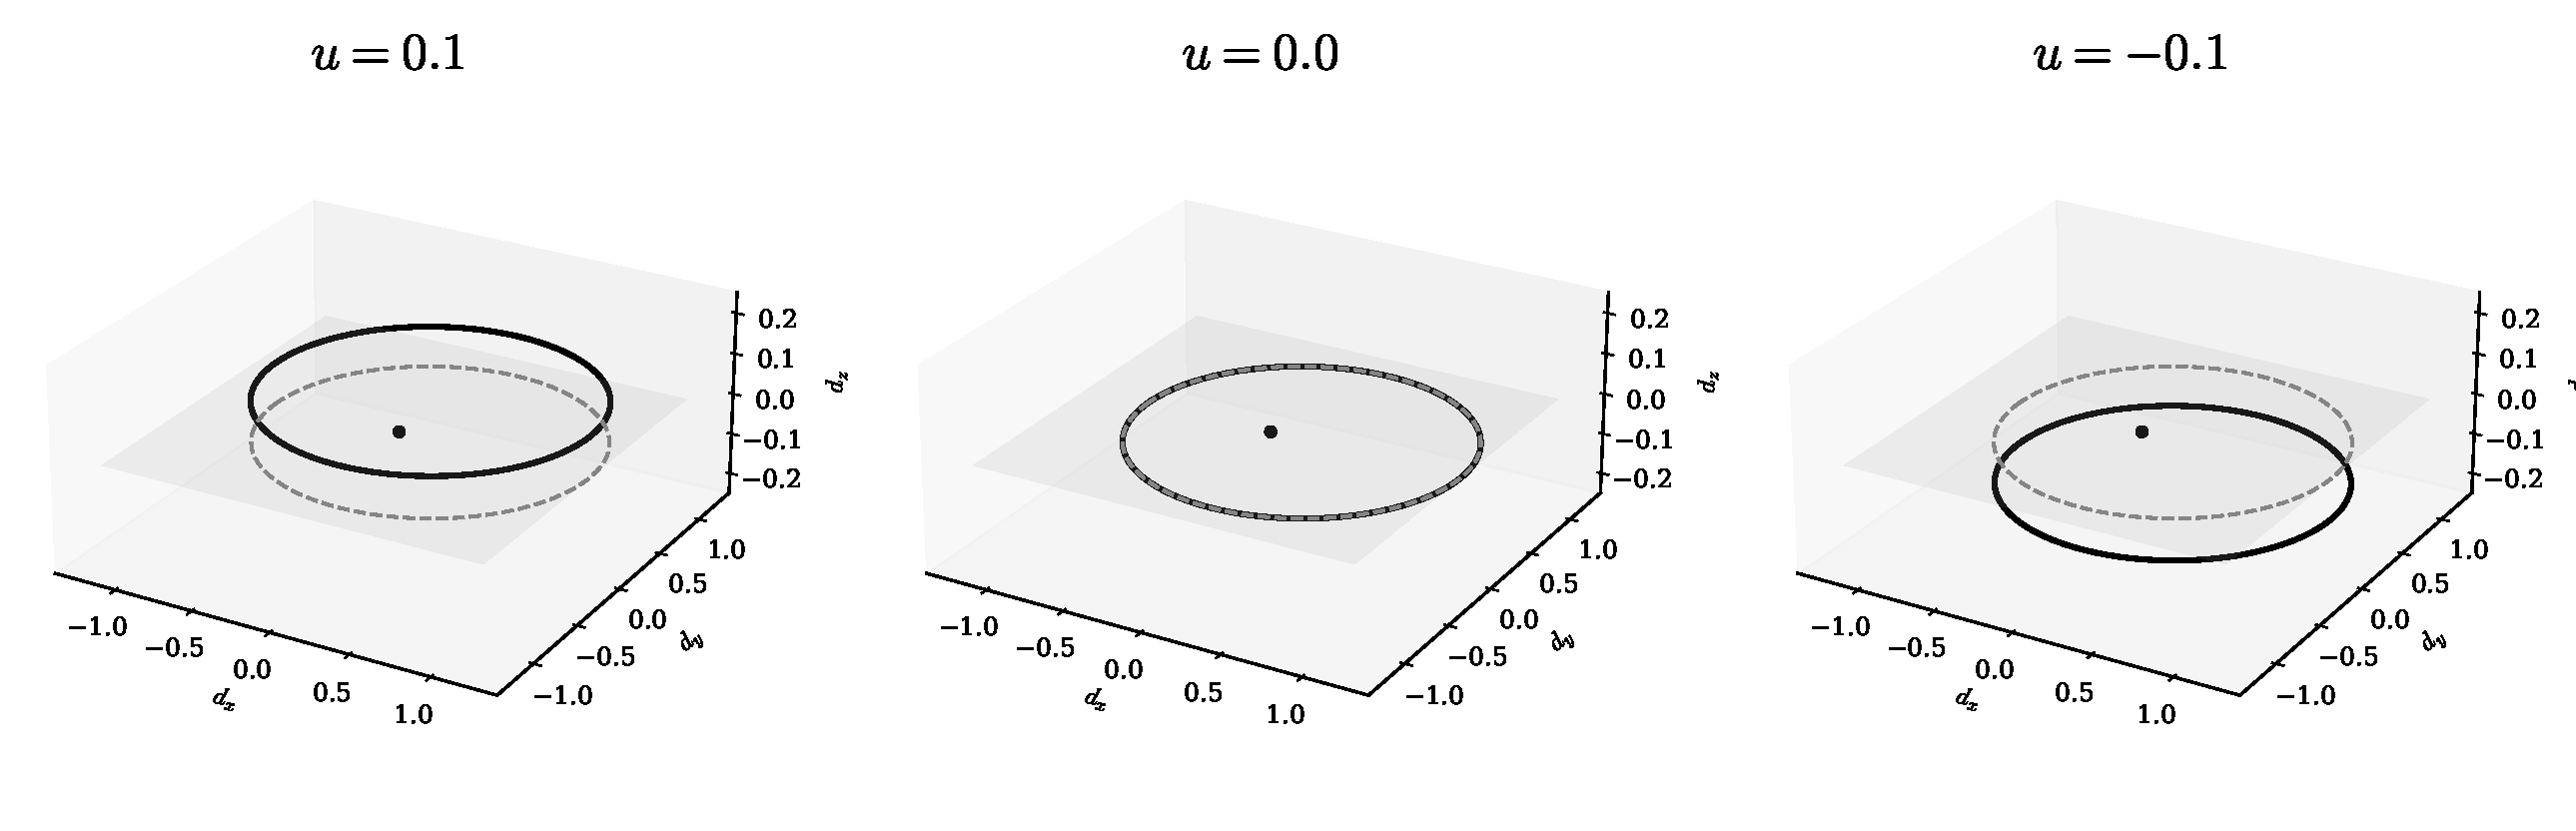
\includegraphics[width=\textwidth]{Figures/onsite_potential/onsite_dvector_3D.pdf}
    \caption{Three-dimensional trajectories of the vector
$\mathbf d(k)$ for the SSH model with a staggered on-site potential for
$u=-0.1$, $u=0$, and $u=0.1$. For $u=0$, the trajectory lies in the
$d_x$--$d_y$ plane and is characterized by the winding number defined in
\cref{eq:winding_number}. Introducing a finite on-site potential
displaces the trajectory out of the plane by a constant amount
$d_z=u$.}
    \label{fig:onsite_winding}
\end{figure}

For the chiral-symmetric SSH model (\(u=0\)), the vector
\(\mathbf d(k)\) can be completely described by the polar angle

\[
\phi(k)=\tan^{-1}\!\left(\frac{d_y(k)}{d_x(k)}\right),
\]

whose total change over the Brillouin zone determines the winding
number. The presence of the \(u\sigma_z\) term removes this planar
constraint by introducing a finite \(d_z\)-component. Consequently,
\(\mathbf d(k)\) can no longer be parametrized by a single angular
variable, and the planar winding number is no longer well defined. The
three-dimensional trajectory therefore provides a more appropriate
geometric representation of the effect of the staggered on-site
potential and the breaking of chiral symmetry.


\begin{table}[htbp]
\centering
\caption{Comparison of the topological and spectral properties of the chiral-symmetric SSH model and the SSH model with a staggered on-site potential.}
\label{tab:sshcomparison}
\renewcommand{\arraystretch}{1.3}
\begin{tabular}{@{}lcc@{}}
\toprule
\textbf{Property} & \textbf{SSH Model} & \textbf{SSH + On-site Potential} \\
\midrule
Chiral symmetry & Preserved & Broken \\
Hamiltonian form & Purely off-diagonal & Contains diagonal $u\sigma_z$ term \\
Energy Spectrum & Symmetric about $E=0$ & Generally not symmetric about $E=0$ \\
$d_z$ component & $0$ & $u$ \\
$\mathbf{d}(k)$ trajectory & Planar & Three-dimensional \\
Winding number & Well-defined & Undefined  \\
Edge-state energy & Zero energy & Shifted away from zero \\
Edge-state localization & Localized & Remain localized \\

\bottomrule
\end{tabular}
\end{table}

\clearpage

\section{Conclusion}

In this work, the Su--Schrieffer--Heeger (SSH) model was comprehensively investigated using a tight-binding framework to elucidate the fundamental interplay between symmetry and topology in one-dimensional electronic systems. Starting from the real-space tight-binding Hamiltonian, we derived the bulk momentum-space representation and mapped it onto the Pauli matrix basis. This vector formulation allowed for an analytical description of the bulk energy dispersion and the determination of the bulk band gap, which continuously closes and reopens at the critical transition point $v=w$. By calculating the topological invariant—the winding number $\nu$—we successfully classified the system into a topologically trivial phase ($\nu=0$ for $v>w$) and a non-trivial phase ($\nu=1$ for $w>v$).

To verify the physical implications of this bulk classification, a finite SSH chain with open boundary conditions was modeled and analyzed via exact numerical diagonalization. In perfect agreement with the bulk--boundary correspondence, the topological phase manifested a pair of mid-gap states localized strongly at the boundaries of the chain. These localized edge states were shown to be a direct consequence of the internal chiral (sublattice) symmetry of the bipartite lattice, which constrains the bulk Hamiltonian to a block off-diagonal structure and strictly pins the edge-state eigenvalues to zero energy. 

Furthermore, we extended the standard SSH model by introducing a staggered on-site potential $\pm u$ to explore the stability of these topological properties. Numerical and analytical treatments revealed that the on-site potential introduces a diagonal $u\sigma_z$ term that completely breaks chiral symmetry, displacing the vector $\mathbf{d}(k)$ out of the two-dimensional plane into a three-dimensional trajectory and rendering the planar winding number ill-defined. Consequently, the edge states lose their spectral protection and shift away from zero energy. Remarkably, however, their spatial boundary localization remains largely intact for small potential strengths, showcasing a nuanced distinction between spectral symmetry protection and spatial confinement.

In summary, this report demonstrates that the SSH model serves as an elegant, foundational platform for understanding topological insulators and phase transitions. On a personal note, this summer research internship has provided an invaluable opportunity to bridge the gap between abstract mathematical concepts—such as topology, chiral symmetry, and Hilbert space decompositions—and concrete physical phenomena. Through the rigorous process of analytical derivations, Python-based numerical modeling, and the synthesis of this \LaTeX{} manuscript, this project has significantly strengthened my theoretical intuition, computational skill set, and scientific communication capabilities, laying a solid foundation for my future research pursuits in theoretical and computational physics.

\clearpage
\section*{Acknowledgements}

I would like to express my sincere gratitude to Dr. Panch Ram, Department of Physics, Indian Institute of Technology (BHU) Varanasi, for giving me the opportunity to undertake this summer research internship and for his invaluable guidance throughout its course. I am deeply grateful for the many insightful and stimulating discussions, his constant encouragement, and his patience in addressing my questions. His mentorship not only helped me develop a strong understanding of the Su–Schrieffer–Heeger (SSH) model and its topological properties but also taught me the importance of approaching physics through careful mathematical reasoning and physical intuition.

I am particularly thankful for the emphasis he placed on understanding the underlying concepts rather than merely obtaining results. The freedom to explore ideas beyond the immediate scope of the project, together with his thoughtful suggestions and constructive feedback, encouraged me to ask deeper questions, develop greater mathematical rigor, and appreciate the fundamental role of symmetry and topology in modern physics. This internship has been an immensely rewarding learning experience that has strengthened my problem-solving skills, deepened my appreciation for rigorous theoretical analysis, and provided me with a strong foundation for future research.









\clearpage
\printbibliography
\addcontentsline{toc}{section}{References}


\clearpage
\appendix
\section{Python Implementations}
The following Python implementations were developed to reproduce all numerical results presented in this report. The programs generate the dispersion relations, winding trajectories, finite-chain spectra, edge-state probability distributions, and the modified SSH model including a staggered on-site potential.

\subsection{Dispersion Relation and Winding Trajectories}

This appendix contains the Python program used to generate the energy dispersion curves and the corresponding winding trajectories presented in \cref{fig:bands_winding}.


This program evaluates the analytical bulk dispersion relation discussed in \cref{sec:ssh_model},
\begin{equation}
E(k)=\pm\sqrt{v^{2}+w^{2}+2vw\cos k},
\end{equation}

and computes the vector

\begin{equation}
\mathbf{d}(k)=
\left(
v+w\cos k,\,
w\sin k
\right),
\end{equation}

for different values of the intracell hopping amplitude \(v\) and intercell hopping amplitude \(w\).
The calculations were performed using the \texttt{NumPy} and \texttt{Matplotlib} libraries.

\begin{lstlisting}[language=Python, caption={Python implementation used to generate the SSH band structure and winding trajectories.}, label={lst:ssh_plot}]
import numpy as np
import matplotlib.pyplot as plt

# Hopping parameters
params = [
    (1.0, 0.0),
    (0.6, 0.4),
    (0.5, 0.5),
    (0.4, 0.6),
    (0.0, 1.0),
]

# Crystal momentum
k = np.linspace(-np.pi, np.pi, 1000)

def dispersion(v, w, k):
    """SSH energy bands."""
    return np.sqrt(v**2 + w**2 + 2*v*w*np.cos(k))

def winding(v, w, k):
    """d-vector components."""
    dx = v + w*np.cos(k)
    dy = w*np.sin(k)
    return dx, dy

fig, ax = plt.subplots(2, 5, figsize=(16,6))

for i, (v, w) in enumerate(params):

    # Dispersion
    E = dispersion(v, w, k)
    ax[0,i].plot(k, E, color='black')
    ax[0,i].plot(k,-E, color='black')
    ax[0,i].set_title(rf"$v={v},\,w={w}$")

    # Winding trajectory
    dx, dy = winding(v, w, k)
    ax[1,i].plot(dx, dy, color='black')
    ax[1,i].scatter(0,0,color='black',s=20)
    ax[1,i].set_aspect('equal')

plt.tight_layout()
plt.savefig("ssh_bands_winding.pdf")
plt.show()
\end{lstlisting}

The program evaluates the analytical expressions derived in \cref{sec:ssh_model} and generates the dispersion curves together with the corresponding winding trajectories for different ratios of the hopping amplitudes.
These plots are used to illustrate the closing and reopening of the bulk band gap and the change in the winding behaviour across the topological phase transition.

\subsection{Finite SSH Chain: Numerical Diagonalization}

This appendix contains the Python program used to construct the finite SSH Hamiltonian with open boundary conditions, perform its numerical diagonalization, and generate the energy spectra and edge-state probability distributions presented in \cref{sec:energy spectra} and \cref{sec:edge_state_probability}.

The Hamiltonian matrix is constructed for a finite chain containing \(N\) unit cells with alternating intracell and intercell hopping amplitudes. The complete set of eigenvalues and orthonormal eigenvectors is obtained using the \texttt{scipy.linalg.eigh()} routine. The probability distribution corresponding to the eigenstate closest to zero energy is then evaluated separately on the \(A\) and \(B\) sublattices.

Calculations were carried out for finite chains with \(N=10\) and \(N=20\) unit cells for several values of the hopping amplitudes in order to illustrate the transition between the trivial and topological phases.

\begin{lstlisting}[language=Python,
caption={Python implementation used to construct and diagonalize the finite SSH Hamiltonian with open boundary conditions and generate the corresponding energy spectra and edge-state probability distributions.},
label={lst:ssh_finite}]

import numpy as np
import matplotlib.pyplot as plt
import scipy.linalg as la

# ------------------------------------------------------------
# Construct the SSH Hamiltonian with open boundary conditions
# ------------------------------------------------------------

def build_ssh_hamiltonian(v, w, N):
    """Return the 2N x 2N SSH Hamiltonian."""

    H = np.zeros((2*N, 2*N))

    for m in range(N):

        # Intracell hopping
        H[2*m, 2*m+1] = v
        H[2*m+1, 2*m] = v

        # Intercell hopping
        if m < N-1:
            H[2*m+1, 2*m+2] = w
            H[2*m+2, 2*m+1] = w

    return H


# ------------------------------------------------------------
# Numerical diagonalization
# ------------------------------------------------------------

def diagonalize(H):
    """Compute eigenvalues and eigenvectors."""

    eigvals, eigvecs = la.eigh(H)

    # Find the smallest positive eigenvalue
    positive_indices = np.where(eigvals > 1e-12)[0]

    if len(positive_indices) == 0:
        raise ValueError("No positive eigenvalues found.")

    idx = positive_indices[0]
    psi = eigvecs[:, idx]

    # Calculate probabilities
    prob = np.abs(psi) ** 2
    prob_A = prob[0::2]
    prob_B = prob[1::2]

    return eigvals, prob_A, prob_B


# ------------------------------------------------------------
# Energy spectrum
# ------------------------------------------------------------

def plot_spectrum(eigvals):

    plt.figure(figsize=(6,4))

    plt.scatter(
        np.arange(len(eigvals)),
        eigvals,
        s=35,
        color="black"
    )

    plt.axhline(0, ls="--", color="gray")

    plt.xlabel("State Index")
    plt.ylabel(r"Energy $E$")

    plt.tight_layout()


# ------------------------------------------------------------
# Edge-state probability distribution
# ------------------------------------------------------------

def plot_probability(prob_A, prob_B):

    cells = np.arange(len(prob_A))
    width = 0.4

    plt.figure(figsize=(7,4))

    plt.bar(
        cells-width/2,
        prob_A,
        width,
        label="A"
    )

    plt.bar(
        cells+width/2,
        prob_B,
        width,
        label="B"
    )

    plt.xlabel("Unit Cell")
    plt.ylabel(r"$|\psi|^2$")

    plt.legend()

    plt.tight_layout()


# ------------------------------------------------------------
# Main program
# ------------------------------------------------------------

parameter_sets = [

    (0.2,1.0,10),
    (0.5,1.0,10),
    (1.0,1.0,10),
    (1.5,1.0,10),

    (0.2,1.0,20),
    (0.5,1.0,20),
    (1.0,1.0,20),
    (1.5,1.0,20),
]

for v, w, N in parameter_sets:

    H = build_ssh_hamiltonian(v, w, N)

    eigvals, prob_A, prob_B = diagonalize(H)

    plot_spectrum(eigvals)

    plot_probability(prob_A, prob_B)





\end{lstlisting}

The program first constructs the finite SSH Hamiltonian as a \(2N\times2N\) Hermitian matrix with open boundary conditions by including alternating intracell (\(v\)) and intercell (\(w\)) hopping amplitudes. The complete eigenspectrum is then obtained through numerical diagonalization using the \texttt{scipy.linalg.eigh()} routine.

For each set of hopping parameters, the code generates two types of numerical results. The first is the complete energy spectrum of the finite chain, illustrating the emergence of near-zero-energy states in the topological phase. The second is the probability distribution associated with the eigenstate closest to zero energy, obtained from the corresponding eigenvector. By separating the probability density on the two sublattices, the calculations demonstrate the localization of the edge states at opposite ends of the chain in the topological regime. The generated figures correspond to those presented in \cref{sec:energy spectra} and \cref{sec:edge_state_probability}.

\subsection{Finite SSH Chain with On-Site Potential}

This appendix contains the Python implementation used to construct and diagonalize the finite SSH Hamiltonian in the presence of an alternating on-site potential. The Hamiltonian is constructed for a finite chain with open boundary conditions,

\begin{align}
\hat H
={}&
v\sum_{m=1}^{N}
\left(
|m,A\rangle\langle m,B|
+
|m,B\rangle\langle m,A|
\right)
+
w\sum_{m=1}^{N-1}
\left(
|m+1,A\rangle\langle m,B|
+
|m,B\rangle\langle m+1,A|
\right)
\nonumber\\[0.5em]
&+
u\sum_{m=1}^{N}
\left(
|m,A\rangle\langle m,A|
-
|m,B\rangle\langle m,B|
\right).
\end{align}

where \(u\) denotes the alternating on-site potential. Numerical diagonalization is performed using the \texttt{scipy.linalg.eigh()} routine. The program generates the complete energy spectrum together with the probability distributions of the positive- and negative-energy edge states for several values of \(u\).

\begin{lstlisting}[
language=Python,
caption={Python implementation used to diagonalize the finite SSH Hamiltonian with an alternating on-site potential and obtain the corresponding energy spectra and edge-state probability distributions.},
label={lst:onsite_open}
]
import numpy as np
import matplotlib.pyplot as plt
import scipy.linalg as la

def ssh_hamiltonian(v, w, u, N):
    H = np.zeros((2*N, 2*N))

    for n in range(N):
        A, B = 2*n, 2*n + 1

        H[A, A] =  u
        H[B, B] = -u

        H[A, B] = H[B, A] = v

        if n < N-1:
            H[B, A+2] = H[A+2, B] = w

    return H


def edge_states(H):

    eigvals, eigvecs = eigh(H)

    pos = np.where(eigvals > 1e-30)[0][0]
    neg = np.where(eigvals < -1e-30)[0][-1]

    Ppos = np.abs(eigvecs[:, pos])**2
    Pneg = np.abs(eigvecs[:, neg])**2

    return (
        eigvals,
        Ppos[0::2], Ppos[1::2],
        Pneg[0::2], Pneg[1::2],
    )


def plot_probability(pA1, pB1, pA2, pB2):

    cells = np.arange(len(pA1))
    width = 0.4

    fig, ax = plt.subplots(1, 2, figsize=(14,5), sharey=True)

    for axis, A, B, title in zip(
        ax,
        [pA1, pA2],
        [pB1, pB2],
        ["Positive Edge State", "Negative Edge State"]
    ):

        axis.bar(cells-width/2, A, width, label="A")
        axis.bar(cells+width/2, B, width, label="B")

        axis.set_title(title)
        axis.set_xlabel("Unit Cell")
        axis.set_xticks(cells)
        axis.grid(alpha=0.5)

    ax[0].set_ylabel(r"$|\psi|^2$")
    ax[0].legend()

    plt.tight_layout()
    plt.show()


def plot_spectrum(eigvals):

    fig, ax = plt.subplots(figsize=(7,5))

    idx = np.arange(len(eigvals))

    pos = np.where(eigvals > 1e-30)[0][0]
    neg = np.where(eigvals < -1e-30)[0][-1]

    ax.scatter(idx, eigvals, s=40)
    ax.scatter([neg, pos],
               [eigvals[neg], eigvals[pos]],
               color="red", s=70)

    ax.axhline(0, ls="--", color="gray")

    ax.set_xlabel("State Index")
    ax.set_ylabel("Energy")
    ax.grid(alpha=0.5)

    plt.tight_layout()
    plt.show()


parameter_sets = [
    (0.2, 1.0, 0.0, 10),
    (0.2, 1.0, 0.1, 10),
    (0.2, 1.0,-0.1, 10),
    (0.2, 1.0, 0.0, 20),
    (0.2, 1.0, 0.1, 20),
    (0.2, 1.0,-0.1, 20),
]

for v, w, u, N in parameter_sets:

    H = ssh_hamiltonian(v, w, u, N)

    eigvals, pA1, pB1, pA2, pB2 = edge_states(H)

    plot_probability(pA1, pB1, pA2, pB2)
    plot_spectrum(eigvals)
\end{lstlisting}


The program constructs the finite SSH Hamiltonian with alternating intracell and intercell hopping amplitudes together with opposite on-site potentials on the two sublattices. Following numerical diagonalization, the complete eigenspectrum is obtained and the positive- and negative-energy edge states are identified. Their probability densities are then evaluated separately on the \(A\) and \(B\) sublattices, illustrating that the edge states remain spatially localized despite their energies shifting away from zero as a consequence of chiral symmetry breaking.

\subsection{SSH Model with On-Site Potential: Three-Dimensional Winding Trajectories}

This appendix contains the Python implementation used to generate the three-dimensional winding trajectories presented in \cref{sec:3d_winding_trajectory}. The program evaluates the modified SSH Hamiltonian in the presence of an alternating on-site potential \(u\),

\begin{equation}
\mathbf d(k)=
\left(
v+w\cos k,\,
w\sin k,\,
u
\right),
\end{equation}

where the additional \(d_z=u\) component shifts the trajectory out of the
\(d_x\)-\(d_y\) plane. The code produces the three-dimensional trajectory together with its projection onto the \(d_x\)-\(d_y\) plane for different values of the on-site potential. Calculations were performed using the \texttt{NumPy} and \texttt{Matplotlib} libraries.

\begin{lstlisting}[language=Python,
caption={Python implementation used to generate the three-dimensional winding trajectories of the SSH model in the presence of an alternating on-site potential.},
label={lst:onsite_winding}]
import numpy as np
import matplotlib.pyplot as plt

# Model parameters
v, w = 0.2, 1.0
onsite_values = [0.1, 0.0, -0.1]

k = np.linspace(-np.pi, np.pi, 800)
dx = v + w*np.cos(k)
dy = w*np.sin(k)

plt.rcParams.update({
    "font.family": "serif",
    "mathtext.fontset": "cm",
    "font.size": 12
})

fig = plt.figure(figsize=(18, 6))

# Plane z = 0
x = np.linspace(-1.2, 1.2, 2)
y = np.linspace(-1.2, 1.2, 2)
X, Y = np.meshgrid(x, y)
Z = np.zeros_like(X)

for i, u in enumerate(onsite_values):

    ax = fig.add_subplot(1, 3, i+1, projection="3d")

    ax.plot(dx, dy, np.full_like(k, u),
            color="black", lw=2.5)

    ax.plot(dx, dy, np.zeros_like(k),
            "--", color="gray", lw=1.5)

    ax.plot_surface(X, Y, Z,
                    color="lightgray",
                    alpha=0.15,
                    edgecolor="none")

    ax.scatter(0, 0, 0, color="black", s=25)

    ax.set(
        xlim=(-1.4, 1.4),
        ylim=(-1.4, 1.4),
        zlim=(-0.25, 0.25),
        xlabel=r"$d_x$",
        ylabel=r"$d_y$",
        zlabel=r"$d_z$"
    )

    ax.set_box_aspect((1, 1, 0.45))
    ax.view_init(elev=25, azim=-60)
    ax.set_title(rf"$u={u}$", fontsize=22)
    ax.grid(False)

fig.subplots_adjust(wspace=0.18)
plt.savefig("onsite_dvector_3D.pdf",
            dpi=600,
            bbox_inches="tight")
plt.show()

\end{lstlisting}

The program evaluates the modified \(\mathbf d(k)\) vector for several values of the alternating on-site potential and illustrates how the winding trajectory is displaced along the \(d_z\)-direction. The projection of the trajectory onto the \(d_x\)-\(d_y\) plane remains unchanged, demonstrating that the additional on-site potential breaks chiral symmetry while preserving the geometrical projection associated with the original SSH model.



\end{document}